\documentclass[a4paper,12pt,twoside]{memoir}

% Castellano
\usepackage[spanish,es-tabla]{babel}
\selectlanguage{spanish}
\usepackage[utf8]{inputenc}
\usepackage[T1]{fontenc}
\usepackage{lmodern} % scalable font
\usepackage{microtype}
\usepackage{placeins}

% DIBUJAR DIAGRAMAS EN LATEX
\usepackage{amsmath}
\usepackage{amssymb}
\usepackage{tikz}
\usepackage{tikz-uml}
\usepackage{pgf-umlsd}
\usetikzlibrary{calc}

% HACER TABLAS LARGAS (e.g.: tabla de requisitos)
\usepackage{pdflscape}
\usepackage{longtable}
\usepackage{threeparttablex}
\usepackage{footnote}
\makesavenoteenv{longtable}

% Ya no es necesario:
% \RequirePackage{xtab}
% \RequirePackage{multirow}
% \RequirePackage{booktabs}
% \RequirePackage[table]{xcolor}

\usepackage{listings}

\definecolor{codegreen}{rgb}{0,0.6,0}
\definecolor{codegray}{rgb}{0.5,0.5,0.5}
\definecolor{codepurple}{rgb}{0.58,0,0.82}
\definecolor{backcolour}{rgb}{0.95,0.95,0.92}
\lstdefinestyle{mystyle}{
    backgroundcolor=\color{backcolour},   
    commentstyle=\color{codegreen},
    keywordstyle=\color{magenta},
    numberstyle=\tiny\color{codegray},
    stringstyle=\color{codepurple},
    basicstyle=\ttfamily\footnotesize,
    breakatwhitespace=false,         
    breaklines=true,                 
    captionpos=b,                    
    keepspaces=true,                 
    numbers=left,                    
    numbersep=5pt,                  
    showspaces=false,                
    showstringspaces=false,
    showtabs=false,                  
    tabsize=2
}
\lstset{style=mystyle}



% Links
\PassOptionsToPackage{hyphens}{url}\usepackage[colorlinks]{hyperref}
\hypersetup{
	allcolors = {red}
}

% Ecuaciones
\usepackage{amsmath}

% Rutas de fichero / paquete
\newcommand{\ruta}[1]{{\sffamily #1}}

% Párrafos
\nonzeroparskip

% Huérfanas y viudas
\widowpenalty100000
\clubpenalty100000

% Evitar solapes en el header
\nouppercaseheads

% Imagenes
\usepackage{graphicx}
\newcommand{\imagen}[2]{
	\begin{figure}[!h]
		\centering
		\includegraphics[width=0.9\textwidth]{#1}
		\caption{#2}\label{fig:#1}
	\end{figure}
	\FloatBarrier
}

\newcommand{\imagenflotante}[2]{
	\begin{figure}%[!h]
		\centering
		\includegraphics[width=0.9\textwidth]{#1}
		\caption{#2}\label{fig:#1}
	\end{figure}
}



% El comando \figura nos permite insertar figuras comodamente, y utilizando
% siempre el mismo formato. Los parametros son:
% 1 -> Porcentaje del ancho de página que ocupará la figura (de 0 a 1)
% 2 --> Fichero de la imagen
% 3 --> Texto a pie de imagen
% 4 --> Etiqueta (label) para referencias
% 5 --> Opciones que queramos pasarle al \includegraphics
% 6 --> Opciones de posicionamiento a pasarle a \begin{figure}
\newcommand{\figuraConPosicion}[6]{%
  \setlength{\anchoFloat}{#1\textwidth}%
  \addtolength{\anchoFloat}{-4\fboxsep}%
  \setlength{\anchoFigura}{\anchoFloat}%
  \begin{figure}[#6]
    \begin{center}%
      \Ovalbox{%
        \begin{minipage}{\anchoFloat}%
          \begin{center}%
            \includegraphics[width=\anchoFigura,#5]{#2}%
            \caption{#3}%
            \label{#4}%
          \end{center}%
        \end{minipage}
      }%
    \end{center}%
  \end{figure}%
}

%
% Comando para incluir imágenes en formato apaisado (sin marco).
\newcommand{\figuraApaisadaSinMarco}[5]{%
  \begin{figure}%
    \begin{center}%
    \includegraphics[angle=90,height=#1\textheight,#5]{#2}%
    \caption{#3}%
    \label{#4}%
    \end{center}%
  \end{figure}%
}
% Para las tablas
\newcommand{\otoprule}{\midrule [\heavyrulewidth]}
%
% Nuevo comando para tablas pequeñas (menos de una página).
\newcommand{\tablaSmall}[5]{%
 \begin{table}
  \begin{center}
   \rowcolors {2}{gray!35}{}
   \begin{tabular}{#2}
    \toprule
    #4
    \otoprule
    #5
    \bottomrule
   \end{tabular}
   \caption{#1}
   \label{tabla:#3}
  \end{center}
 \end{table}
}

%
%Para el float H de tablaSmallSinColores
\usepackage{float}

%
% Nuevo comando para tablas pequeñas (menos de una página).
\newcommand{\tablaSmallSinColores}[5]{%
 \begin{table}[H]
  \begin{center}
   \begin{tabular}{#2}
    \toprule
    #4
    \otoprule
    #5
    \bottomrule
   \end{tabular}
   \caption{#1}
   \label{tabla:#3}
  \end{center}
 \end{table}
}

\newcommand{\tablaApaisadaSmall}[5]{%
\begin{landscape}
  \begin{table}
   \begin{center}
    \rowcolors {2}{gray!35}{}
    \begin{tabular}{#2}
     \toprule
     #4
     \otoprule
     #5
     \bottomrule
    \end{tabular}
    \caption{#1}
    \label{tabla:#3}
   \end{center}
  \end{table}
\end{landscape}
}

%
% Nuevo comando para tablas grandes con cabecera y filas alternas coloreadas en gris.
\newcommand{\tabla}[6]{%
  \begin{center}
    \tablefirsthead{
      \toprule
      #5
      \otoprule
    }
    \tablehead{
      \multicolumn{#3}{l}{\small\sl continúa desde la página anterior}\\
      \toprule
      #5
      \otoprule
    }
    \tabletail{
      \hline
      \multicolumn{#3}{r}{\small\sl continúa en la página siguiente}\\
    }
    \tablelasttail{
      \hline
    }
    \bottomcaption{#1}
    \rowcolors {2}{gray!35}{}
    \begin{xtabular}{#2}
      #6
      \bottomrule
    \end{xtabular}
    \label{tabla:#4}
  \end{center}
}

%
% Nuevo comando para tablas grandes con cabecera.
\newcommand{\tablaSinColores}[6]{%
  \begin{center}
    \tablefirsthead{
      \toprule
      #5
      \otoprule
    }
    \tablehead{
      \multicolumn{#3}{l}{\small\sl continúa desde la página anterior}\\
      \toprule
      #5
      \otoprule
    }
    \tabletail{
      \hline
      \multicolumn{#3}{r}{\small\sl continúa en la página siguiente}\\
    }
    \tablelasttail{
      \hline
    }
    \bottomcaption{#1}
    \begin{xtabular}{#2}
      #6
      \bottomrule
    \end{xtabular}
    \label{tabla:#4}
  \end{center}
}

%
% Nuevo comando para tablas grandes sin cabecera.
\newcommand{\tablaSinCabecera}[5]{%
  \begin{center}
    \tablefirsthead{
      \toprule
    }
    \tablehead{
      \multicolumn{#3}{l}{\small\sl continúa desde la página anterior}\\
      \hline
    }
    \tabletail{
      \hline
      \multicolumn{#3}{r}{\small\sl continúa en la página siguiente}\\
    }
    \tablelasttail{
      \hline
    }
    \bottomcaption{#1}
  \begin{xtabular}{#2}
    #5
   \bottomrule
  \end{xtabular}
  \label{tabla:#4}
  \end{center}
}



\definecolor{cgoLight}{HTML}{EEEEEE}
\definecolor{cgoExtralight}{HTML}{FFFFFF}

%
% Nuevo comando para tablas grandes sin cabecera.
\newcommand{\tablaSinCabeceraConBandas}[5]{%
  \begin{center}
    \tablefirsthead{
      \toprule
    }
    \tablehead{
      \multicolumn{#3}{l}{\small\sl continúa desde la página anterior}\\
      \hline
    }
    \tabletail{
      \hline
      \multicolumn{#3}{r}{\small\sl continúa en la página siguiente}\\
    }
    \tablelasttail{
      \hline
    }
    \bottomcaption{#1}
    \rowcolors[]{1}{cgoExtralight}{cgoLight}

  \begin{xtabular}{#2}
    #5
   \bottomrule
  \end{xtabular}
  \label{tabla:#4}
  \end{center}
}




\graphicspath{ {./img/} }

% Capítulos
\chapterstyle{bianchi}
\newcommand{\capitulo}[2]{
	\setcounter{chapter}{#1}
	\setcounter{section}{0}
	\setcounter{figure}{0}
	\setcounter{table}{0}
	\chapter*{#2}
	\addcontentsline{toc}{chapter}{#2}
	\markboth{#2}{#2}
}

% Apéndices
\renewcommand{\appendixname}{Apéndice}
\renewcommand*\cftappendixname{\appendixname}

\newcommand{\apendice}[1]{
	%\renewcommand{\thechapter}{A}
	\chapter{#1}
}

\renewcommand*\cftappendixname{\appendixname\ }

% Formato de portada
\makeatletter
\usepackage{xcolor}
\newcommand{\tutor}[1]{\def\@tutor{#1}}
\newcommand{\course}[1]{\def\@course{#1}}
\definecolor{cpardoBox}{HTML}{E6E6FF}
\def\maketitle{
  \null
  \thispagestyle{empty}
  % Cabecera ----------------
\noindent
\includegraphics[width=\textwidth]{cabecera}\vspace{1cm}%
  \vfill
  % Título proyecto y escudo informática ----------------
  \colorbox{cpardoBox}{%
    \begin{minipage}{.8\textwidth}
      \vspace{.5cm}\Large
      \begin{center}
      \textbf{TFG del Grado en Ingeniería Informática}\vspace{.6cm}\\
      \textbf{\LARGE\@title{}}
      \end{center}
      \vspace{.2cm}
    \end{minipage}

  }%
  \hfill\begin{minipage}{.20\textwidth}
    
\includegraphics[width=\textwidth]{escudoInfor}
  \end{minipage}
  \vfill
  % Datos de alumno, curso y tutores ------------------
  \begin{center}%
  {%
    \noindent\LARGE
    Presentado por \@author{}\\ 
    en Universidad de Burgos --- \@date{}\\
    Tutor: \@tutor{}\\
  }%
  \end{center}%
  \null
  \cleardoublepage
  }
\makeatother


% Datos de portada
\title{Algoritmos y mazmorras \\Documentación Técnica}
\author{Elsa Tolín Carrasco}
\tutor{Jesús Alonso Abad y José Manuel Galán Ordax}
\date{\today}

\begin{document}

\maketitle



\cleardoublepage



%%%%%%%%%%%%%%%%%%%%%%%%%%%%%%%%%%%%%%%%%%%%%%%%%%%%%%%%%%%%%%%%%%%%%%%%%%%%%%%%%%%%%%%%



\frontmatter


\clearpage

% Indices
\tableofcontents

\clearpage

\listoffigures

\clearpage

\listoftables

\clearpage

\mainmatter

\appendix

\apendice{Plan de Proyecto Software}

\section{Introducción}
El desarrollo del presente proyecto se ha extendido durante 3 años por motivos personales, pero el tiempo de desarrollo efectivo es menor. Es por este motivo que, para desarrollar la planificación se va a tener el cuenta el tiempo productivo.

Para el desarrollo de este proyecto se ha hecho una planificación utilizando la metodología Scrum. Se ha dividido el trabajo por sprints y para poder llevar un seguimiento de las tareas a realizar, se ha hecho uso de el método Kanban. Para poder llevar a cabo esta metodología, se ha hecho uso de la aplicación web Jira. En el método Kanban se utiliza un tablón dividido por varias columnas, cada una especifica un estado de la tarea, y se va actualizando en este tablero según van progresando las tareas.


\section{Planificación temporal}
Por lo mencionado anteriormente, aunque no haya sido el tiempo real de desarrollo, se va a dividir la planificación de sprints efectivos de tres semanas.

\subsection{Fases del desarrollo}

\begin{enumerate}
    \item Pruebas de concepto
    \item Primera Fase
        \begin{enumerate}
            \item Investigación del motor
            \item Investigación de algoritmos de generación procedimental
            \item Implementación en el motor
        \end{enumerate}
    \item Segunda Fase
        \begin{enumerate}
            \item Preparación del servidor
            \item Preparación del front-end con Unity
            \item Preparación de ejecutable
            \item Tests
            \item Documentación
        \end{enumerate}
\end{enumerate}



\subsection{Sprint 1}
Durante este sprint, se llevo a cabo una investigación de las posibles herramientas y lenguajes de programación que se podrían utilizar para desarrollar la idea del proyecto. Por ello se realizaron distintas pruebas de proyecto para comprobar qué problemas y qué ventajas se podrían encontrar durante el desarrollo. 
\begin{itemize}
    \item Java: Construcción de un prototipo desde cero en java con el algoritmo de Wilson
    \item C\# y .NET: Construcción de un prototipo desde cero con C\# y .NET.
\end{itemize}

\subsection{Sprint 2}
Durante este sprint, tras la investigación y las pruebas de concepto se comenzó a investigar la posibilidad de usar un motor gráfico como Unity. 
\begin{itemize}
    \item Aprendizaje sobre Unity: Se realizó un aprendizaje de este motor ya que es complejo y se carecía de experiencia previa con esta herramienta.
    \item Preparación del entorno: Se creó el proyecto en el motor y se preparó la primera escena
\end{itemize}

\subsection{Sprint 3}
En este sprint se trabajó en la estructura y en el algoritmo para poder generar el laberinto. Se necesitó de mucha investigación para aprender sobre cómo realizar estos pasos en Unity.
\begin{itemize}
    \item Desarrollo del la escena para el menú y para el juego
    \item Búsqueda de un algoritmo sencillo para generar el laberinto
    \item Implementación del algoritmo
\end{itemize}

\subsection{Sprint 4}
Durante el desarrollo de este sprint se evaluaron los siguientes pasos y se comenzó a la <<Segunda Fase>> mencionada anteriormente. Se busca un nuevo diseño y se investiga como construir un servidor para conectarlo con el videojuego.
\begin{itemize}
    \item Aprendizaje sobre como preparar el servidor
    \item Creación de la estructura base del servidor
    \item Implementación básica del servidor
    \item Implementación de la adaptación del algoritmo de Prim
\end{itemize}

\subsection{Sprint 5}
Tras la preparación del diseño del servidor y comenzar con su implementación básica, este siguiente sprint tiene como foco implementar en Unity el videojuego. En esta segunda fase el papel de Unity cambia a ser el encargado de dibujar los laberintos. En este sprint también se continua desarrollando algoritmos.
\begin{itemize}
    \item Creación de las escenas necesarias para la interfaz de usuario
    \item Implementación del sistema para dibujar el laberinto
    \item Implementación de la adaptación del algoritmo de Kruskal
    \item Implementación de un DevContainer y se añade Docker a la arquitectura 
    \item Cambio de SQLite a MongoDB
\end{itemize}

\subsection{Sprint 6}
En este sprint se continuó con el desarrollo de algoritmos de generación procedimental y se realizó un notebook de python para comparar sus tiempos de ejecución.
\begin{itemize}
    \item Implementación de la adaptación del algoritmo de DFS
    \item Implementación de la adaptación del algoritmo del Autómata celular
    \item Implementación de la adaptación del algoritmo del Eller
    \item Implementación de la adaptación del algoritmo del Teselación
    \item Implementación de la adaptación del algoritmo del Aldous Broder
    \item Implementación de la adaptación del algoritmo del Árbol binario
    \item Desarrollo en notebook para obtener gráficas para comparar los tiempos de ejecución
\end{itemize}

\subsection{Sprint 7}
Tras realizar la implementación de los algoritmos se preparó el ejecutable y se realizaron pruebas para buscar errores, tras esto se arreglaron los errores encontrados.
\begin{itemize}
    \item Preparación de ejecutables
    \item Solución de errores
\end{itemize}

\subsection{Sprint 8}
Una vez terminado el proyecto se comenzó a desarrollar la documentación del proyecto. Durante este sprint se desarrolló la memoria.

\subsection{Sprint 9}
Tras desarrollar la memoria se realizó la documentación de los anexos del proyecto.

\section{Estudio de viabilidad}
Se va a proceder a realizar el estudio de viabilidad del proyecto. Este estudio no es representativo de un estudio de viabilidad de un videojuego, esto es porque este proyecto se ha centrado en el desarrollo visto desde un programador, no se tienen en cuenta el desarrollo artístico ya que se ha hecho uso de los recursos de la comunidad gratuitos.


\subsection{Viabilidad económica}
En esta sección se va realizar un análisis de los costes financieros que supone el desarrollo del presente proyecto. Para realizar este estudio, aunque el tiempo real de desarrollo han sido tres años, se tendrá en cuenta el tiempo de desarrollo efectivo. En otras palabras, se va a estudiar la viabilidad económica para un periodo efectivo. Los cálculos se realizarán como si se tratase de una nueva empresa con un único empleado, durante un periodo de 27 semanas.

También hay que tener en cuenta que en el caso de Unity, si el último ejercicio fiscal de los ingresos fueron superiores a 100\,000 dolares estadounidenses, se tiene la obligación de comprar la edición profesional de Unity~\cite{unity}. Como no se comercializa el juego, no se necesita tener en cuenta estos gastos. También se va a presuponer que el proyecto es el primero desarrollado con Unity por lo que no hay precedentes que obliguen a comprar la licencia profesional de Unity.

Para poder valorar la viabilidad económica se van a evaluar dos aspectos: los costes y los beneficios. En este caso, se asumirá que el proyecto lo lleva a cabo una empresa con liquidez suficiente como para que no sea necesaria una financiación.

\subsubsection{Costes por recursos}
En primer lugar, se van a analizar los costes derivados de los recursos del \textit{software} y \textit{hardware} que se han utilizado durante el desarrollo.

Las licencias utilizadas han sido gratuitas, y se listarán más adelante en consideración de un desarrollo futuro en el que se requiera obtener un plan de pago. 

Como ya se ha mencionado al inicio de esta sección, aunque la duración del proyecto han sido tres años, vamos a tener en cuenta el tiempo efectivo, por lo que estos cálculos se van a efectuar para un proyecto cuyo periodo de desarrollo ha durado 27 semanas, que equivalen a, aproximadamente, 7 meses.

\begin{itemize}
    \item \textbf{Hardware:}\\ 
    Durante el desarrollo de esta aplicación se ha hecho uso de 1 ordenador portátil. El modelo es MSI Raider GE66 12UH-005ES, este equipo tiene actualmente un precio de 3\,098,86 € y se espera amortizar en 5 años~\cite{portatil}.
    Su coste anual de amortización será: 
    \[
        \frac{3\,098,86\ \text{€}}{5\ \text{años}} \approx 619,77\ \text{€/año}
    \]

    \item \textbf{Software:}\\
    Se ha utilizado una licencia de sistema operativo Windows 11 Pro. Tiene un valor de 199 € mediante medios oficiales~\cite{windows}. Dado que tiene una vida útil de 4 años, se espera amortizar en este tiempo.
    \[
        \frac{199,00\ \text{€}}{4\ \text{años}} \approx 49,75\ \text{€/año}
    \]
\end{itemize}

De esta forma, el coste anual derivado de recursos queda definido en la Tabla \ref{CostResources}.

\vspace{1em}
\begin{table}[h!]
        \caption{Coste anual por recursos.}
	\label{CostResources}
	\centering
	\begin{tabular}{ l  c }
		\toprule
		\textbf{Recurso} & \textbf{Coste anual} \\ \midrule
		Windows 11 Pro & 49,75 €\\
		Portátil & 619,77 € \\
		Unity & 0,00 €\\
		\midrule
		\textbf{Total:} & 669,52 € \\
		\bottomrule
	\end{tabular}
\end{table}


\subsubsection{Costes de personal}
Para simplificar las fórmulas a continuación, utilizaremos las siguientes abreviaturas:
\begin{itemize}
    \item \textbf{SBA}: Salario Bruto Anual (jornada parcial)
    \item \textbf{SBM}: Salario Bruto Mensual
    \item \textbf{CASS}: Contribución Anual a la Seguridad Social
    \item \textbf{CMSS}: Contribución Mensual a la Seguridad Social
    \item \textbf{CP}: Coste en Personal
\end{itemize}

Al realizar estas estimaciones, se va a considerar una empresa pequeña de un único empleado, como se ha mencionado anteriormente. Se va a asumir también, que la duración ha sido de 7 meses efectivos y ha sido desarrollado por un empleado de categoría <<Junior>>. El sueldo anual bruto promedio se encuentra alrededor de unos 25\,000~€ con una jornada completa~\cite{salario}. Para formalizar sus condiciones, se va a considerar que es un contrato a 30 horas a la semana con 12 pagas anuales.

\[
\text{SBA} = \text{25\,000~€}  \cdot \frac{\text{30 horas}}{\text{40 horas}} = \text{18\,750~€}
\]


Con esto obtenemos el salario bruto mensual: 
\[
\text{SBM} = \frac{\text{18\,750~€}}{\text{12 pagas}} = \text{1\,562,5~€}
\]

Para obtener el coste en personal hay que sumarle el salario bruto del empleado, calculamos la contribución anual a la seguridad social~\cite{seguridadsocial} por parte de la empresa.
Esta se compone de 5 costes:
\begin{enumerate}
    \item  Contigencias comunes: 23,60\%
    \item Desempleo: 5,5\%
    \item Fogasa: 0,2\%
    \item Formación profesional 0,6\%
    \item Mecanismo de Equidad Intergeneracional 0,58\%
\end{enumerate}
Haciendo que la contribución sea un 30,48\% del total.
\[
\text{CASS} = 25\,000\ \text{€} \times 0.3048 = 7\,620\ \text{€}
\]

\[
\text{CMSS} = \frac{7\,620\ \text{€}}{12} \approx 635\ \text{€/mes}
\]

El coste en personal total sería el siguiente: 

\[
\text{CP} = \text{SBM} + \text{CMSS}
\]

\[
\text{CP} = \text{1\,562,5 €} + \text{635 €} = \text{2\,197,5 €}
\]

\subsubsection{Coste total}

Considerando todos los gastos anteriores, durante un periodo de 7 meses, se calcula el coste total del proyecto (v. Tabla \ref{Costproject}).

\[
\text{CP (7 meses)} = \text{2\,197,5 €} \cdot 7 \text{ meses} = \text{15\,322,5 €}
\]

\begin{table}[H]
        \caption{Coste total del proyecto}
	\label{Costproject}
	\centering
	\begin{tabular}{ l  c }
		\toprule
		\textbf{Concepto} & \textbf{Coste} \\ \midrule
		Personal & 15\,322,5 €\\
		\textit{Hardware} & 361,53  € \\
		\textit{Software} & 29,02 €\\
		Otros & 0,00 €\\
		
		\midrule
		\textbf{Coste Total del proyecto:} & 15\,713,05 € \\
		\bottomrule
	\end{tabular}
\end{table}


\subsection{Viabilidad legal}

En esta sección se analizará la viabilidad legal del proyecto, revisando las licencias asociadas a cada una de las dependencias utilizadas. Es crucial garantizar que todas las licencias sean compatibles con el uso previsto del software, especialmente cuando se busca elegir la más restrictiva posible para asegurar el cumplimiento legal.

\subsubsection{Licencias de Unity}

Para el desarrollo de este proyecto se han utilizado las siguientes licencias relacionadas con Unity:
\begin{itemize}
    \item \textbf{Unity}: Licencia gratuita. Para más información, se puede consultar el siguiente enlace: \url{https://support.unity.com/hc/en-us/categories/201268913-Licenses}.
    \item \textbf{Elementos de interfaz gráfica de usuario}: Licencia para uso personal y comercial disponible en: \url{https://mandinhart.itch.io/garden-cozy-kit-uigui-buttons-and-icons}.
\end{itemize}

\subsubsection{Dependencias de Python}

Las dependencias de Python utilizadas en este proyecto y sus respectivas licencias\footnote{Es importante destacar que toda la información referente a las licencias de las dependencias de Python se puede consultar fácilmente en \url{https://pypi.org/}, lo cual facilita la verificación y actualización constante de las licencias utilizadas en el proyecto.} se detallan en la Tabla \ref{tab:python-licenses}. Nos servirán para poder determinar qué licencia debemos emplear en el repositorio.

\subsubsection{Licencia del proyecto}

La elección de la licencia más restrictiva es esencial para asegurar que el uso del \textit{software} cumple con todas las restricciones y obligaciones legales. En el análisis, las licencias BSD-3-Clause y Apache 2.0 son las más restrictivas entre las utilizadas. Ambas requieren que se incluya una copia de la licencia original, manteniendo así el reconocimiento de los derechos de los autores originales. La licencia Apache 2.0 añade, además, una cláusula de patentes, lo que puede incrementar las restricciones de uso en comparación con la BSD-3-Clause~\cite{licencia1,licencia2}.

Por lo tanto, para maximizar la compatibilidad y asegurar el cumplimiento legal, se recomienda adoptar las prácticas y obligaciones definidas por la licencia Apache 2.0, dado que incluye las restricciones adicionales sobre patentes y proporciona una mayor cobertura en términos de cumplimiento legal.

\subsubsection{Implicaciones legales y cumplimiento}

Es fundamental que los desarrolladores comprendan las implicaciones legales de cada licencia utilizada en el proyecto. A continuación, se presentan algunas directrices para cumplir con las obligaciones legales al redistribuir o modificar el \textit{software}:

\begin{itemize}
    \item \textbf{Incluir una copia de la licencia}. Al distribuir el \textit{software}, es obligatorio incluir una copia de la licencia elegida.
    \item \textbf{Mantener los avisos de derechos de autor}. No se deben eliminar ni modificar los avisos de derechos de autor presentes en el código fuente.
    \item \textbf{Proporcionar modificaciones bajo la misma licencia}. Si se realizan modificaciones a una dependencia con una licencia \textit{copyleft}, como la Apache 2.0, es necesario redistribuir dichas modificaciones bajo la misma licencia.
    \item \textbf{Informar sobre las licencias aplicables}. La documentación del proyecto debe incluir información clara sobre las licencias aplicables a cada parte del \textit{software}.
\end{itemize}

Siguiendo estas directrices, se asegura que el proyecto cumple con todas las obligaciones legales y se minimiza el riesgo de infracciones de licencias.

\vspace{1cm}

% TABLA DE LICENCIAS
\begin{ThreePartTable}
% Nota al pie
\renewcommand\TPTminimum{\textwidth}
\begin{TableNotes}
\footnotesize % letra pequeña (tamaño letra de pie de página)
    \item[a] \url{https://mit-license.org/}
    \item[b] \url{http://www.apache.org/licenses/}
    \item[c] \url{https://opensource.org/license/bsd-2-clause}
    \item[d] \url{https://opensource.org/license/BSD-3-clause}
    \item[e] \url{https://www.isc.org/licenses/}
    \item[f] \url{https://docs.python.org/3/license.html}
\end{TableNotes}

% Comienza la tabla
\begin{longtable}{llp{7cm}}
    \caption{Dependencias de Python y sus licencias}\label{tab:python-licenses}\\
    % ESTRUCTURA
    \toprule
    \textbf{Dependencia} & \textbf{Versión} & \textbf{Licencia} \\ \midrule
    \endfirsthead
    \caption*{Dependencias de Python y sus licencias (continuación)}\\
    \toprule
    \textbf{Dependencia} & \textbf{Versión} & \textbf{Licencia} \\ \midrule
    \endhead
    \bottomrule
    \endfoot
    \bottomrule
    \insertTableNotes  % Notas
    \endlastfoot
    % DATOS DE LA TABLA
    annotated-types & 0.6.0 & MIT License\tnote{a} \\ 
    anyio & 4.3.0 & MIT License\tnote{a} \\ 
    debugpy & 1.8.1 & MIT License\tnote{a} \\ 
    executing & 2.0.1 & MIT License\tnote{a} \\ 
    fastapi & 0.110.1 & MIT License\tnote{a} \\ 
    h11 & 0.14.0 & MIT License\tnote{a} \\ 
    jedi & 0.19.1 & MIT License\tnote{a} \\ 
    parso & 0.8.4 & MIT License\tnote{a} \\ 
    platformdirs & 4.2.0 & MIT License\tnote{a} \\ 
    pure-eval & 0.2.2 & MIT License\tnote{a} \\ 
    pydantic & 2.7.0 & MIT License\tnote{a} \\ 
    pydantic\_core & 2.18.1 & MIT License\tnote{a} \\ 
    six & 1.16.0 & MIT License\tnote{a} \\ 
    stack-data & 0.6.3 & MIT License\tnote{a} \\ 
    toml & 0.10.2 & MIT License\tnote{a} \\ 
    asttokens & 2.4.1 & Apache License 2.0\tnote{b} \\ 
    beanie & 1.25.0 & Apache License 2.0\tnote{b} \\ 
    lazy-model & 0.2.0 &  Apache License 2.0\tnote{b} \\ 
    motor & 3.4.0 &  Apache License 2.0\tnote{b} \\ 
    packaging & 24.0 & Apache License 2.0\tnote{b} ~y BSD-2-Clause License\tnote{c} \\ 
    pymongo & 4.6.3 &  Apache License 2.0\tnote{b} \\ 
    python-dateutil & 2.9.0.post0 &  Apache License 2.0\tnote{b} \\ 
    tornado & 6.4 &  Apache License 2.0\tnote{b} \\ 
    click & 8.1.7 & BSD-3-Clause License\tnote{d} \\ 
    comm & 0.2.2 & BSD-3-Clause License\tnote{d} \\ 
    idna & 3.7 & BSD-3-Clause License\tnote{d} \\ 
    ipykernel & 6.29.4 & BSD-3-Clause License\tnote{d} \\ 
    ipython & 8.23.0 & BSD-3-Clause License\tnote{d} \\ 
    jupyter\_client & 8.6.1 & BSD-3-Clause License\tnote{d} \\ 
    jupyter\_core & 5.7.2 & BSD-3-Clause License\tnote{d} \\ 
    matplotlib-inline & 0.1.6 & BSD-3-Clause License\tnote{d} \\ 
    prompt-toolkit & 3.0.43 & BSD-3-Clause License\tnote{d} \\ 
    psutil & 5.9.8 & BSD-3-Clause License\tnote{d} \\ 
    pyzmq & 25.1.2 & BSD-3-Clause License\tnote{d} \\ 
    starlette & 0.37.2 & BSD-3-Clause License\tnote{d} \\ 
    traitlets & 5.14.2 & BSD-3-Clause License\tnote{d} \\ 
    uvicorn & 0.29.0 & BSD-3-Clause License\tnote{d} \\ 
    decorator & 5.1.1 & BSD-2-Clause License\tnote{c} \\ 
    nest-asyncio & 1.6.0 & BSD-2-Clause License\tnote{c} \\ 
    Pygments & 2.17.2 & BSD-2-Clause License\tnote{c} \\ 
    dnspython & 2.6.1 & ISC License\tnote{e} \\ 
    pexpect & 4.9.0 & ISC License\tnote{e} \\ 
    ptyprocess & 0.7.0 & ISC License\tnote{e} \\ 
    typing\_extensions & 4.11.0 & Python Software Foundation License\tnote{f} \\ 
    sniffio & 1.3.1 & Apache License 2.0\tnote{b} ~y MIT License\tnote{a} \\
\end{longtable}
\end{ThreePartTable}




\apendice{Especificación de Requisitos}

\section{Introducción}
Para poder llevar a cabo un proyecto de \textit{sofware}, se necesitan tener requisitos especificados, con esto se podrá realizar el desarrollo, usando estos requisitos como guía.

En este apartado se van a abarcar las especificaciones de requisitos y los casos de uso que reflejarán el funcionamiento del producto de \textit{software} desarrollado.

\section{Objetivos generales}
Este proyecto tiene como objetivo principal la generación de laberintos que puedan ser navegables por el usuario. Los objetivos para llevar a cabo el proyecto son los siguientes:
\begin{enumerate}
    \item Obtener laberintos que sean navegables.
    \item Utilizar varios algoritmos de generación procedimental para generar los laberintos.
    \item Usar la arquitectura cliente-servidor para poder almacenar datos del videojuego.
    \item Utilizar el protocolo HTTP para que el servidor se comunique con Unity.
    \item Calcular los tiempos de ejecución de estos algoritmos y compararlos.
    \item Generar una imagen del contenido con Docker para que se pueda alojar fácilmente en un servidor externo.
\end{enumerate}


\section{Catalogo de requisitos}

\subsection{Requisitos funcionales}
Los requisitos funcionales definen el comportamiento que se espera por la aplicación. Para este proyecto se han redactado los siguientes:

%    \item \textbf{RF1 - }
%		\begin{itemize}
%  			\item \textbf{RF1.1}: 
%			\item \textbf{RF1.2}: 
%			\item \textbf{RF1.3}:
%		\end{itemize}

\begin{itemize}
	\item \textbf{RF1 - Laberintos navegables}
		\begin{itemize}
  			\item \textbf{RF1.1}: El usuario puede navegar por el laberinto con el objeto <<Player>> utilizando las teclas W, A, S, D.
            \item \textbf{RF1.2}: El usuario colisiona con los muros, es decir, no puede atravesar paredes.
			\item \textbf{RF1.3}: El usuario puede tener acceso a la pantalla anterior con un botón de retorno.
            \item \textbg{RF1.4}:
		\end{itemize}
    \item \textbf{RF2 - Gestión del menú principal}
		\begin{itemize}
  			\item \textbf{RF2.1}: El usuario puede navegar por el menú principal
			\item \textbf{RF2.2}: El usuario puede abandonar el juego.
			\item \textbf{RF2.3}: El usuario puede moverse a la siguiente pantalla a través del menú.
		\end{itemize}
    \item \textbf{RF3 - Gestión del menú secundario}
		\begin{itemize}
  			\item \textbf{RF3.1}: El usuario puede navegar el menú secundario.
			\item \textbf{RF3.2}: El usuario puede seleccionar el algoritmo que desea usar para la generación del laberinto.
			\item \textbf{RF3.3}: El usuario debe poder acceso a la pantalla anterior con un botón de retorno.
		\end{itemize}
    \item \textbf{RF4 - Gestión de los laberintos generados}
		\begin{itemize}
  			\item \textbf{RF4.1}: La aplicación puede almacenar los laberintos con sus dimensiones y  semilla generados.
		\end{itemize}
    \item \textbf{RF5 - Generación de laberintos parametrizables}
		\begin{itemize}
  			\item \textbf{RF5.1}: El usuario puede introducir el ancho del laberinto a generar si el algoritmo lo permite.
            \item \textbf{RF5.2}: El usuario puede introducir el largo del laberinto a generar si el algoritmo lo permite.
            \item \textbf{RF5.3}: El usuario puede introducir el número de iteraciones si el algoritmo lo permite.
            \item \textbf{RF5.4}: El usuario puede introducir la semilla de la generación procedimental.
		\end{itemize}
\end{itemize}

\subsection{Requisitos no funcionales}
Los requisitos no funcionales engloban aquellos que no especifican el funcionamiento de la aplicación, van a definir el comportamiento del producto.
\begin{itemize}
    \item \textbf{RNF1 - Velocidad de respuesta}
		\begin{itemize}
  			\item \textbf{RNF1.1}: La carga del laberinto debe ser lo más rápida posible.
		\end{itemize}
    \item \textbf{RNF2 - Transparencia}
		\begin{itemize}
  			\item \textbf{RNF2.1}: Los cambios futuros deberán ser transparentes al usuario, ya que no hay necesidad de que conozca cómo funciona internamente el programa
		\end{itemize}
    \item \textbf{RNF3 - Usabilidad}
		\begin{itemize}
  			\item \textbf{RNF3.1}: La navegación por la aplicación debe de ser cómoda.
            \item \textbf{RNF3.2}: La navegación por los laberintos debe de ser intuitiva.
		\end{itemize}
\end{itemize}


\section{Especificación de requisitos}
\begin{figure}[!h]  
    \centering  
    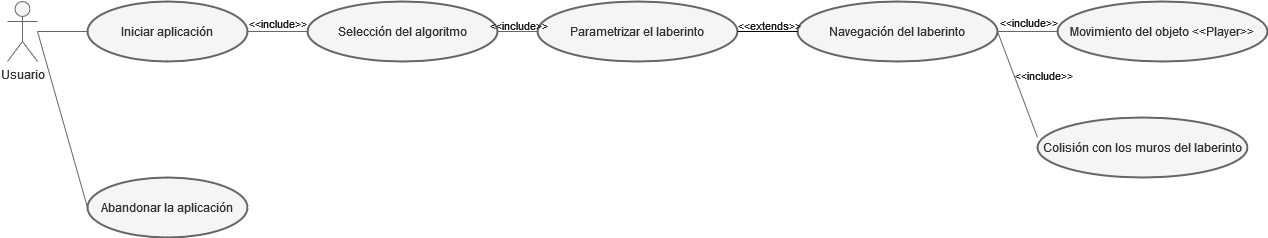
\includegraphics[width=\textwidth]{img/CasosUso.png}  
    \caption{Caso de uso de la aplicación.}  
    \label{fig:CasosDeUso}
\end{figure}
\begin{table}[p]
	\centering
	\begin{tabularx}{\linewidth}{ p{0.21\columnwidth} p{0.71\columnwidth} }
			\toprule
			\textbf{CU-1}    & \textbf{Iniciar aplicación}\\
			\toprule
			\textbf{Versión}              & 1.0    \\
			\textbf{Autor}                & Elsa Tolín \\
			\textbf{Requisitos asociados} & RF-2.1, RF-2.3 \\
			\textbf{Descripción}          & Este caso de uso permite visualizar el menú principal y seleccionar el botón de arranque\\
			\textbf{Precondición}         & Arranque de la aplicación\\
			\textbf{Acciones}             &
			\begin{enumerate}
					\def\labelenumi{\arabic{enumi}.}
					\tightlist
					\item Acceder a la página del menú principal
					\item Pulsar botón
				\end{enumerate}\\
			\textbf{Postcondición}        & Redirección al menú secundario\\
			\textbf{Excepciones}          &  \\
			\textbf{Importancia}          & Alta\\
			\bottomrule
		\end{tabularx}
	\caption{CU-1 Inicio de aplicación.}
\end{table}

\begin{table}[p]
	\centering
	\begin{tabularx}{\linewidth}{ p{0.21\columnwidth} p{0.71\columnwidth} }
			\toprule
			\textbf{CU-2}    & \textbf{Selección del algoritmo}\\
			\toprule
			\textbf{Versión}              & 1.0    \\
			\textbf{Autor}                & Elsa Tolín \\
			\textbf{Requisitos asociados} & RF-3.1, RF-3.2 \\
			\textbf{Descripción}          & El usuario puede seleccionar el algoritmo que desea probar en la aplicación\\
			\textbf{Precondición}         & Seleccionar el botón <<comenzar>> en la pantalla del menú principal\\
			\textbf{Acciones}             &
			\begin{enumerate}
					\def\labelenumi{\arabic{enumi}.}
					\tightlist
					\item Acceder al menú secundario
					\item Pulsar botón del algoritmo deseado
				\end{enumerate}\\
			\textbf{Postcondición}        & Redirección a la pantalla de generación de laberintos. \\
			\textbf{Excepciones}          &  \\
			\textbf{Importancia}          & Alta\\
                \textbf{Nota}          & Este caso de uso se aplica para todos los algoritmos que puede seleccionar el usuario\\
			\bottomrule
		\end{tabularx}
	\caption{CU-2 Selección del algoritmo.}
\end{table}

\begin{table}[p]
	\centering
	\begin{tabularx}{\linewidth}{ p{0.21\columnwidth} p{0.71\columnwidth} }
			\toprule
			\textbf{CU-3}    & \textbf{Parametrizar el laberinto}\\
			\toprule
			\textbf{Versión}              & 1.0    \\
			\textbf{Autor}                & Elsa Tolín \\
			\textbf{Requisitos asociados} & RF-5, RF-5.1, RF-5.2, RF-5.3, RF-5.4 \\
			\textbf{Descripción}          & Se puede parametrizar el tamaño del laberinto, ya sea por ancho y largo o por número de iteraciones\\
			\textbf{Precondición}         & Seleccionar el botón del algoritmo que se va a probar\\
			\textbf{Acciones}             &
			\begin{enumerate}
					\def\labelenumi{\arabic{enumi}.}
					\tightlist
					\item Acceder al menú secundario
					\item Selección del botón según el algoritmo que se vaya a probar
                    \item Introducir ancho y largo en las cajas de texto
                    \item Introducir semilla (opcional)
                    \item Pulsar el botón de <<Generar mazmorra>>
				\end{enumerate}\\
			\textbf{Postcondición}        & Se genera el laberinto \\
			\textbf{Excepciones}          &  En caso de que sea el algoritmo de teselación o de árbol binario se pedirán al usuario las iteraciones. Si los datos introducidos no son correctos pedirá al usuario volverlos a introducir. Si el campo de la semilla no se completa se utilizará una semilla generada por el programa.\\
			\textbf{Importancia}          & Alta\\
			\bottomrule
		\end{tabularx}
	\caption{CU-3 Parametrizar el laberinto.}
\end{table}


\begin{table}[p]
	\centering
	\begin{tabularx}{\linewidth}{ p{0.21\columnwidth} p{0.71\columnwidth} }
			\toprule
			\textbf{CU-4}    & \textbf{Navegación del laberinto}\\
			\toprule
			\textbf{Versión}              & 1.0    \\
			\textbf{Autor}                & Elsa Tolín \\
			\textbf{Requisitos asociados} & RF-1, RF-1.1, RF-1.2 \\
			\textbf{Descripción}          & El usuario se puede mover por el laberinto en tiempo real.\\
			\textbf{Precondición}         & Pulsar el botón de <<Generar mazmorra>>\\
			\textbf{Acciones}             &
			\begin{enumerate}
					\def\labelenumi{\arabic{enumi}.}
					\tightlist
					\item El usuario pulsa una de las teclas (W A S D) se desplaza
				\end{enumerate}\\
			\textbf{Postcondición}        & 
            \begin{enumerate}
					\def\labelenumi{\arabic{enumi}.}
					\tightlist
					\item El usuario no ha atravesado ni se ha introducido en un muro
                    \item El usuario ha cambiado su posición dentro del laberinto
				\end{enumerate}\\
			\textbf{Excepciones}          & Colisiona con un muro\\
			\textbf{Importancia}          & Alta\\
			\bottomrule
		\end{tabularx}
	\caption{CU-4 Navegación del laberinto}
\end{table}


\begin{table}[p]
	\centering
	\begin{tabularx}{\linewidth}{ p{0.21\columnwidth} p{0.71\columnwidth} }
			\toprule
			\textbf{CU-5}    & \textbf{Abandonar la aplicación}\\
			\toprule
			\textbf{Versión}              & 1.0    \\
			\textbf{Autor}                & Elsa Tolín \\
			\textbf{Requisitos asociados} & RF1.3, RF-2.2 \\
			\textbf{Descripción}          & El usuario puede abandonar la aplicación y que la ventana se cierre automáticamente\\
			\textbf{Precondición}         & \\
			\textbf{Acciones}             &
			\begin{enumerate}
					\def\labelenumi{\arabic{enumi}.}
					\tightlist
					\item El usuario se encuentra en la pantalla de exploración de laberinto
                    \item El usuario pulsa sobre el botón <<volver>>
                    \item El usuario se encuentra en la pantalla de selección de algoritmo
                    \item El usuario pulsa sobre el botón <<volver>>
                    \item El usuario se encuentra en la pantalla principal
                    \item El usuario pulsa sobre el botón <<salir>>
				\end{enumerate}\\
			\textbf{Postcondición}        & Cierre de la aplicación\\
			\textbf{Excepciones}          & \\
			\textbf{Importancia}          & Alta\\
			\bottomrule
		\end{tabularx}
	\caption{CU-5 Abandonar la aplicación}
\end{table}


\apendice{Especificación de diseño}

\section{Introducción}

La especificación de diseño es un componente fundamental en la creación de sistemas robustos y escalables. En esta sección se detallará el diseño de los datos, secuencias y arquitectura del \textit{software} desarrollado. Esto permite visualizar de forma sencilla la estructura y los datos que componen el proyecto.

\section{Diseño de datos}

En este proyecto se utiliza una base de datos NoSQL implementada mediante Beanie\footnote{La documentación oficial se puede consultar en el siguiente enlace: \url{https://beanie-odm.dev/}}, un Object Document Mapper (ODM) para Python, que permite una interacción sencilla y eficiente con MongoDB. A continuación, se describen detalladamente las estructuras de datos empleadas y su implementación.

\subsection{Modelo de datos}

El modelo de datos se define mediante la clase \texttt{DungeonResponse}, la cual hereda de \texttt{Document} y \texttt{BaseModel}. Esta combinación permite utilizar las ventajas de un ODM y las validaciones de datos ofrecidas por Pydantic. Para utilizar este modelo de datos en nuestra aplicación, es necesario seguir una serie de pasos. Primero, se debe conectar a la base de datos MongoDB y luego realizar las operaciones CRUD (\textit{e.g.}, crear, leer, actualizar o eliminar) sobre los documentos \texttt{DungeonResponse}.

\noindent A continuación, se presenta la definición de la clase que modela el documento.

\vspace{1em} % Dejar un espacio de margen

\begin{lstlisting}[language=Python]
from beanie import Document
from typing import List, Dict, Any
from pydantic import BaseModel

class DungeonResponse(Document, BaseModel):
    algorithm: str
    seed: int
    parameters: Dict[str, Any]
    maze: List[List[int]]

\end{lstlisting}

\subsection{Descripción de los campos}

\begin{itemize}
    \item \textbf{algorithm}: este campo de tipo \texttt{str} almacena el nombre del algoritmo utilizado para generar el laberinto. Es fundamental para identificar el método específico de generación empleado.
    \item \textbf{seed}: de tipo \texttt{int}, este campo guarda la semilla utilizada para la generación del laberinto. El uso de una semilla asegura la reproducibilidad de los laberintos generados.
    \item \textbf{parameters}: este es un diccionario (\texttt{Dict[str, Any]}) que contiene parámetros adicionales utilizados por el algoritmo de generación. La flexibilidad de este campo permite adaptarse a diversas configuraciones algorítmicas.
    \item \textbf{maze}: este campo es una lista de listas de enteros (\texttt{List[List[int]]}) que representa la estructura del laberinto generado, donde cada entero indica el tipo de celda correspondiente.
\end{itemize}


 \begin{figure}[h!]
 \centering
 \begin{tikzpicture}
     \tikzstyle{every node}=[draw, shape=rectangle, rounded corners, align=center, minimum width=6cm]
     \node (dr) {DungeonResponse};
     \node[below, yshift=-0.34cm] (fields) {algorithm: str\\ seed: int\\ parameters: Dict[str, Any]\\ maze: List[List[int]]};
 \end{tikzpicture}
 \caption{Diagrama del nodo DungeonResponse}
 \end{figure}


\subsection{Ventajas del diseño NoSQL}

El uso de una base de datos NoSQL, específicamente MongoDB, proporciona diversas ventajas en este contexto, a saber:

\begin{itemize}
    \item \textbf{Flexibilidad en el esquema}. La estructura flexible de documentos en MongoDB permite modificar el modelo de datos sin necesidad de migraciones complejas.
    \item \textbf{Escalabilidad}. MongoDB está diseñado para manejar grandes volúmenes de datos y proporciona escalabilidad horizontal mediante la partición de datos (\textit{sharding}).
    \item \textbf{Consultas rápidas}. Las consultas y agregaciones en MongoDB son rápidas y eficientes, lo cual es crucial para aplicaciones que requieren respuestas en tiempo real.
\end{itemize}


\section{Diseño procedimental}
En esta sección se describen los procedimientos utilizados en el proyecto para controlar el flujo de información que hay entre el usuario y el proyecto. Para poder ilustrarlos, se diseñan varios diagramas de secuencia siguiendo la normativa UML. 

En primer lugar, se va a analizar el flujo de información que se da cuando se genera un laberinto nuevo; es decir, cuando el laberinto no está inicialmente almacenado en la base de datos del servidor. Corresponde con la figura \ref{fig:LaberintoNuevo}.

En segundo lugar, se va a analizar el caso en el que el laberinto sí se encuentra ya generado en la base de datos. Corresponde con la figura \ref{fig:LaberintoAlmacenado}.

\begin{figure}[H]
    \centering  
    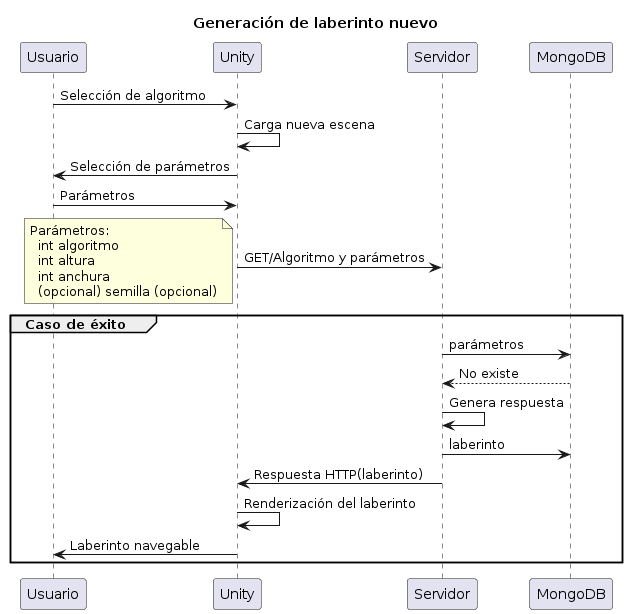
\includegraphics[width=\textwidth]{img/LaberintoNuevo.png}  
    \caption{Diagrama de secuencias de un laberinto nuevo.}  
    \label{fig:LaberintoNuevo}
\end{figure}

\begin{figure}[H]
    \centering  
    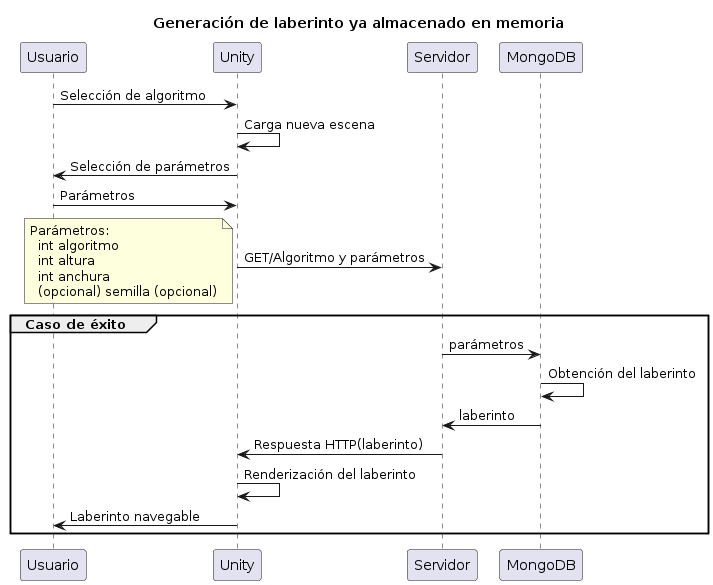
\includegraphics[width=\textwidth]{img/LaberintoYaAlmacenado.png}  
    \caption{Diagrama de secuencias de un laberinto ya almacenado.}  
    \label{fig:LaberintoAlmacenado}
\end{figure}



\section{Diseño arquitectónico}

El diseño arquitectónico de la aplicación se basa en una arquitectura cliente-servidor, donde el cliente está desarrollado en Unity, el servidor utiliza FastAPI y la base de datos es MongoDB. Este enfoque permite una comunicación eficiente y estructurada entre los componentes, asegurando un flujo de datos coherente y una gestión centralizada de la lógica de negocio. 

\subsection{Arquitectura cliente-servidor}

La arquitectura cliente-servidor empleada se divide en dos componentes principales:

\begin{itemize}
    \item \textbf{Cliente}. La interfaz gráfica y la lógica de presentación de la aplicación se desarrollan en Unity. Este componente es responsable de interactuar con el usuario final y de enviar solicitudes al servidor.
    \item \textbf{Servidor}. Este componente maneja las solicitudes del cliente, procesa la lógica de negocio y realiza operaciones sobre la base de datos. FastAPI, un \textit{framework} web moderno y rápido para Python, se utiliza para construir las API que facilitan la comunicación entre el cliente y el servidor. Por otro lado, en el lado del servidor localizamos también la base de datos MongoDB, que se utiliza para almacenar de manera eficiente los datos necesarios para la aplicación.
\end{itemize}

Esta arquitectura vista en conjunto no es monolítica, pero si se miran por separado cliente y servidor, cada uno de ellos son dos monolitos.

A continuación, en la Figura \ref{fig:arquitectura}, se presenta un diagrama que ilustra la arquitectura cliente-servidor.

\begin{figure}[!h]
    \centering
    \includegraphics[width=0.75\textwidth]{img/cliente_servidor.png}
    \caption[Arquitectura cliente-servidor.]{Arquitectura cliente-servidor\protect\footnotemark.}
    \label{fig:arquitectura}
\end{figure}

\footnotetext{Diagrama creado empleando iconos vectoriales de libre acceso desde la página \url{https://www.flaticon.es/}}

\subsection{FastAPI y REST}

FastAPI es un \textit{framework} web moderno para Python que permite la creación rápida y eficiente de API RESTful. Este \textit{framework} es conocido por su alto rendimiento y facilidad de uso, permitiendo a los desarrolladores definir y gestionar \textit{endpoints} de manera declarativa.

\subsubsection{REST}

REST (Representational State Transfer) es un estilo arquitectónico para diseñar servicios web que utilizan HTTP como protocolo de comunicación. Los principios de REST incluyen:

\begin{itemize}
    \item \textbf{Statelessness}. Cada solicitud del cliente al servidor debe contener toda la información necesaria para entender y procesar la solicitud.
    \item \textbf{Resource-Based}. Los recursos (datos) son identificados por URLs y pueden ser manipulados usando los métodos HTTP estándar (GET, POST, PUT, DELETE).
    \item \textbf{Representation}. Los recursos son representados en formatos estándar como JSON o XML.
\end{itemize}

\subsubsection{OpenAPI y Swagger}

FastAPI soporta de manera nativa la generación de documentación OpenAPI y Swagger. OpenAPI es una especificación que define una forma estándar de describir y documentar las API RESTful. Swagger es un conjunto de herramientas para la creación de documentación interactiva de API basadas en la especificación OpenAPI.

FastAPI genera automáticamente la documentación de la API en formato OpenAPI, y proporciona una interfaz web interactiva mediante Swagger UI, donde los desarrolladores pueden explorar y probar los \textit{endpoints} de la API.

\vspace{1em}

\begin{figure}[H]
    \centering
    \includegraphics[width=0.75\linewidth]{img/tech_arch.png} % Ignorar error, no afecta
    \caption{Tecnologías empleadas en la arquitectura}
    \label{fig:enter-label}
\end{figure}


\subsection{Modelo-Vista-Controlador}

El patrón de diseño Modelo-Vista-Controlador (MVC) se utiliza para estructurar la aplicación de manera que se separen claramente los intereses de datos, interfaz de usuario y control de flujo~\cite{mvc}. Este patrón se implementa de la siguiente manera:

\begin{itemize}
    \item \textbf{Modelo}: representa los datos y la lógica de negocio de la aplicación. En este caso, incluye las clases y estructuras que interactúan con la base de datos MongoDB, como \texttt{DungeonResponse}.
    \item \textbf{Vista}: maneja la representación visual de los datos y la interacción con el usuario. Unity actúa como la vista en esta arquitectura, proporcionando una interfaz gráfica interactiva.
    \item \textbf{Controlador}: interpreta las entradas del usuario y las convierte en acciones sobre el modelo. FastAPI sirve como el controlador, gestionando las solicitudes del cliente, aplicando la lógica de negocio y respondiendo adecuadamente.
\end{itemize}

El siguiente diagrama muestra la implementación del patrón MVC en la arquitectura.

\vspace{1em}

\begin{figure}[H]
    \centering
    \begin{tikzpicture}[node distance=3cm, auto, every node/.style={align=center}]
    
        % Nodes
        \node[rectangle, draw, fill=green!30] (view) {Vista};
        
        \node[rectangle, draw, fill=yellow!30, right of=view, node distance=5cm] (model) {Modelo};
        \node at ($(model)+(1.5,0)$) {
\includegraphics[height=1cm]{img/bbdd.png}};
    
        
        \node[rectangle, draw, fill=orange!30, below of=view, node distance=5cm] (controller) {Controlador};
        
        \node[left of=view, node distance=4cm] (user){
\includegraphics[height=1cm]{img/avatar.png}};
    
        % Arrows
        \draw[->] (view) -- node[anchor=east] {Llama} (controller);
        \draw[->] (controller) -- node[anchor=west] {Manipula} (model);
        \draw[->] (model) -- node[anchor=south] {Dispara eventos} (view);
        \draw[->, dashed] (user) -- node[anchor=south] {Interacción} (view);
    \end{tikzpicture}

    \caption{Patrón Modelo-Vista-Controlador}
    \label{fig:mvc}
\end{figure}

\subsection{Estrategia y Método Plantilla}
En el diseño del servidor se utilizan los patrones de diseño Estrategia y Método Plantilla para mejorar tanto la modularidad como la reutilización del código. Estos patrones permiten definir algoritmos específicos de manera concreta, mientras que las partes comunes se establecen en una clase base, facilitando la extensión del diseño con nuevos algoritmos sin modificar el código existente.

El patrón de diseño Estrategia es un patrón de diseño de comportamiento que define una familia de algoritmos, hace que se coloque cada uno de estos algoritmos en una clase separada, es decir, se encapsulan, y se hacen intercambiables~\cite{strategyPattern}. 

El patrón de diseño Método Plantilla es un patrón de diseño de comportamiento, este define el esqueleto de un algoritmo en la superclase pero también permite que las subclases sobrescriban pasos del algoritmo sin cambiar su estructura~\cite{templateMethodPattern}.

En el caso de este proyecto, cada algoritmo de generación procedimental es una estrategia concreta, no se redefinen al completo si no que cada uno hace uso de las partes comunes que están definidas en la clase base y las partes específicas en las clases hijas. De esta forma se mejora la modularidad del código, se reutiliza y se reduce la duplicidad de código. 

Al hacer uso de estos patrones se favorece el principio SOLID Open-Closed. Este propicia la extensión del diseño con nuevos algoritmos sin necesidad de modificar el código existente, haciendo un diseño abierto para extensión pero cerrado para la modificación~\cite{solidOpenClosed}. También se ve favorecido el principio de sustitución de Liskov, este permite que cualquier algoritmo de una subclase pueda sustituir a otro de una superclase sin alterar el comportamiento del programa, así se garantiza que las estrategias sean consistentes~\cite{liskovSubstitutionPrinciple}.

\apendice{Documentación técnica de programación}

\section{Introducción}

En este apartado se va a detallar la estructura del proyecto, las partes que lo componen y la función de cada una. El código final de la aplicación se encuentra dentro de \texttt{/SegundaFase}, el resto de directorios se mantienen como partes del repositorio(\url{https://github.com/etc99/algoritmosYmazmorras}) a modo de histórico de fases previas por las que ha pasado el proyecto antes de tomar la aproximación actual.

\section{Manual del programador}

El código del proyecto se divide entre dos partes principales; una para la aplicación de Unity, incluida en \texttt{/AlgoritmosYMazmorras}; y la parte del servidor de laberintos contenida en \texttt{/Mazmorras}.

\subsection{\texttt{/AlgoritmosYMazmorras}}
Este directorio contiene todo lo relativo a la aplicación de Unity. Sigue la estructura de un proyecto común de Unity.

\subsubsection{\texttt{/Assets}}
Contiene los recursos utilizados en el proyecto. En este directorio se encuentran los \textit{scripts} que establecen los comportamiento de los distintos componentes del juego. También contiene las escenas del juego, así como distintos recursos gráficos, de audio y de texturas utilizados en el juego. Además contiene los distintos \_Prefabs\_ creados para el proyecto.

\subsubsection{\texttt{/Packages}}
Contiene los paquetes utilizados por Unity para el proyecto. Normalmente no hay necesidad de modificar nada de este directorio debido a que el propio Unity ya lo gestiona.

\subsubsection{\texttt{/Library}}
En este directorio se encuentran los archivos generados por Unity en la compilación del juego. Este directorio no es necesario que tenga seguimiento por Git.

\subsubsection{\texttt{/ProjectSettings}}
Este directorio contiene la configuración del proyecto, así como configuración específica del editor de Unity.


\subsection{\texttt{/Mazmorras}}
En este directorio está contenido el servidor de Python junto con los distintos generadores de laberintos, así como de su persistencia en la base de datos de MongoDB.

También contiene ficheros Dockerfile y docker-compose con las que levantar la aplicación en un entorno de contenedores de Docker.

\subsubsection{\texttt{/.devcontainer}}
Esta carpeta contiene los archivos de configuración para el uso de la tecnología de los devcontainers. Está compuesto por un fichero Dockerfile para configurar la imagen del servidor a utilizar en el contenedor de desarrollo, un fichero \texttt{docker-compose.yml} que contiene la configuración con la que lanzar los distintos contenedores de la aplicación para el desarrollo y un fichero \texttt{devcontainer.json} con configuración propia de la tecnología de los devcontainers.

\subsubsection{\texttt{/src}}
Dentro de este directorio está contenido el código que compone el servidor de laberintos.

El fichero \texttt{requirements.txt} contiene las dependencias de bibliotecas externas de nuestro proyecto de Python.

El servidor del backend junto a sus endpoints están declarados dentro del fichero \texttt{app.py}. Desde aquí será donde se manejarán las peticiones realizadas al servidor.

Para lanzar el servidor más cómodamente utilizando uvicorn se ha creado un \textit{script} de nombre \texttt{main.py}.

\subsubsection{\texttt{/dungeon\_api}}

Es la carpeta con los componentes principales del funcionamiento del servidor.

El directorio \texttt{/dungeon\_controllers} contiene módulos que se encargan de la generación de los laberintos y su persistencia en la base de datos. Estos son utilizados en el manejo de peticiones del servidor.

El otro subdirectorio es \texttt{/dungeon\_generators}, que contienen los generadores de laberintos de cada uno de los algoritmos implementados. Para implementarlos se ha recurrido a un enfoque de programación orientada a objetos para añadir funcionalidades que faciliten su serialización y configuración. Todos los generadores heredan de \texttt{DungeonBase}, que provee una interfaz común para los generadores. Está contenido en \texttt{dungeon\_base.py}.

Para la gestión del almacenamiento en MongoDB de los laberintos se usan los modelos de \texttt{/models}. Los modelos definidos aquí dan la estructura que seguirán las entidades almacenadas en la base de datos.


\section{Compilación, instalación y ejecución del proyecto}
Para poder ejecutar este proyecto se tienen que preparar dos partes, el servidor y el cliente, en este caso Unity. En esta sección se va a explicar como preparar ambas partes para poder desarrollar el proyecto.

\subsection{Instalación de Unity}

Unity tiene soporte para ciertos sistemas operativos, entre ellos están
\begin{enumerate}
    \item Windows 7,8,10,11 
    \item macOs X 10.13+
    \item CentOS 7
    \item Rocky
    \item Ubuntu 18.04, 20.04, 22.04
\end{enumerate}

Para poder realizar la instalación del motor gráfico, primero se necesita realizar la descarga de Unity Hub. En el caso de Windows y macOS se necesitaría proceder con los siguientes pasos:
\begin{enumerate}
    \item Acceder a la web de Unity \url{https://unity.com/es/download}.
    \item Desde esa URL se descarga Unity Hub.
    \item Proceder con el proceso del instalador de la ventana de \texttt{setup}.
\end{enumerate}

Al abrir Unity Hub por primera vez, pide el inició de sesión con tu cuenta de Unity, si no se tiene una cuenta previamente se necesita crearla.
Tras esto, en la ventana de unity hub, en el menú de la derecha aparecen distintos botones, entre ellos el botón de <<Installs>> donde aparecerá automáticamente el inicio de descarga de Unity como se muestra en la figura \ref{fig:InstallsUnity}.

\begin{figure}[!h]  
    \centering  
    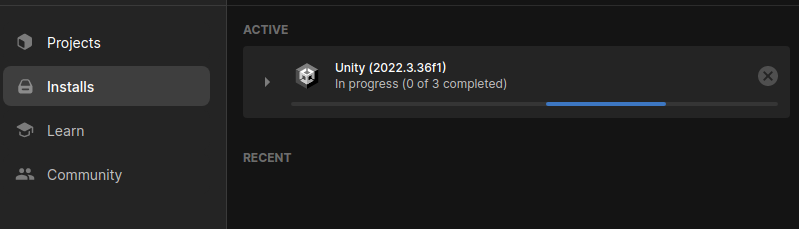
\includegraphics[width=\textwidth]{img/InstallsUnity.png}  
    \caption{Pestaña de instalación de Unity en UnityHub.}  
    \label{fig:InstallsUnity}
\end{figure}

Es recomendable para poder visualizar y trabajar con los \textit{scripts} de Unity instalar Visual Studio Community
Tras la instalación anterior se puede realizar desde el Unity, Edit>Preferences y desde ahí se cambia la herramienta externa.

Tras esto solo quedaría exportar el proyecto a Unity. Unity va a pedir que se instale una versión previa y es porque este proyecto se hizo con la versión \texttt{2021.3.25f1}. 
\begin{figure}[!h]  
    \centering  
    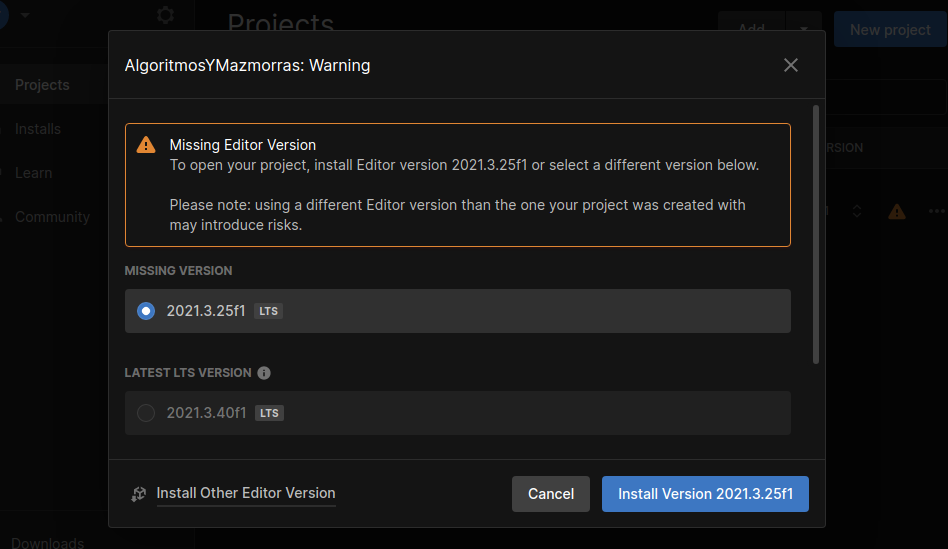
\includegraphics[width=\textwidth]{img/UnityInstallVersion.png}  
    \caption{Pestaña de instalación de nueva versión en Unity.}  
    \label{fig:UnityInstallVersion}
\end{figure}

\subsection{Instalación de Docker}

Para instalar docker primero se necesita obtener de la página de descargas, se puede escoger la versión del siguiente enlace \url{https://docs.docker.com/desktop/release-notes/} y se obtendrá el instalador.
Tras esto sólo quedaría seguir los pasos del instalador. Tras la instalación se necesita ejecutar con permisos administrador.

En máquinas con Windows, es necesario habilitar WSL~\cite{wslContainers}, el subsistema Linux para Windows, para realizarlo se puede hacer desde Docker, como se muestra en la figura \ref{fig:dockerdashboard}.

\begin{figure}[!h]  
    \centering  
    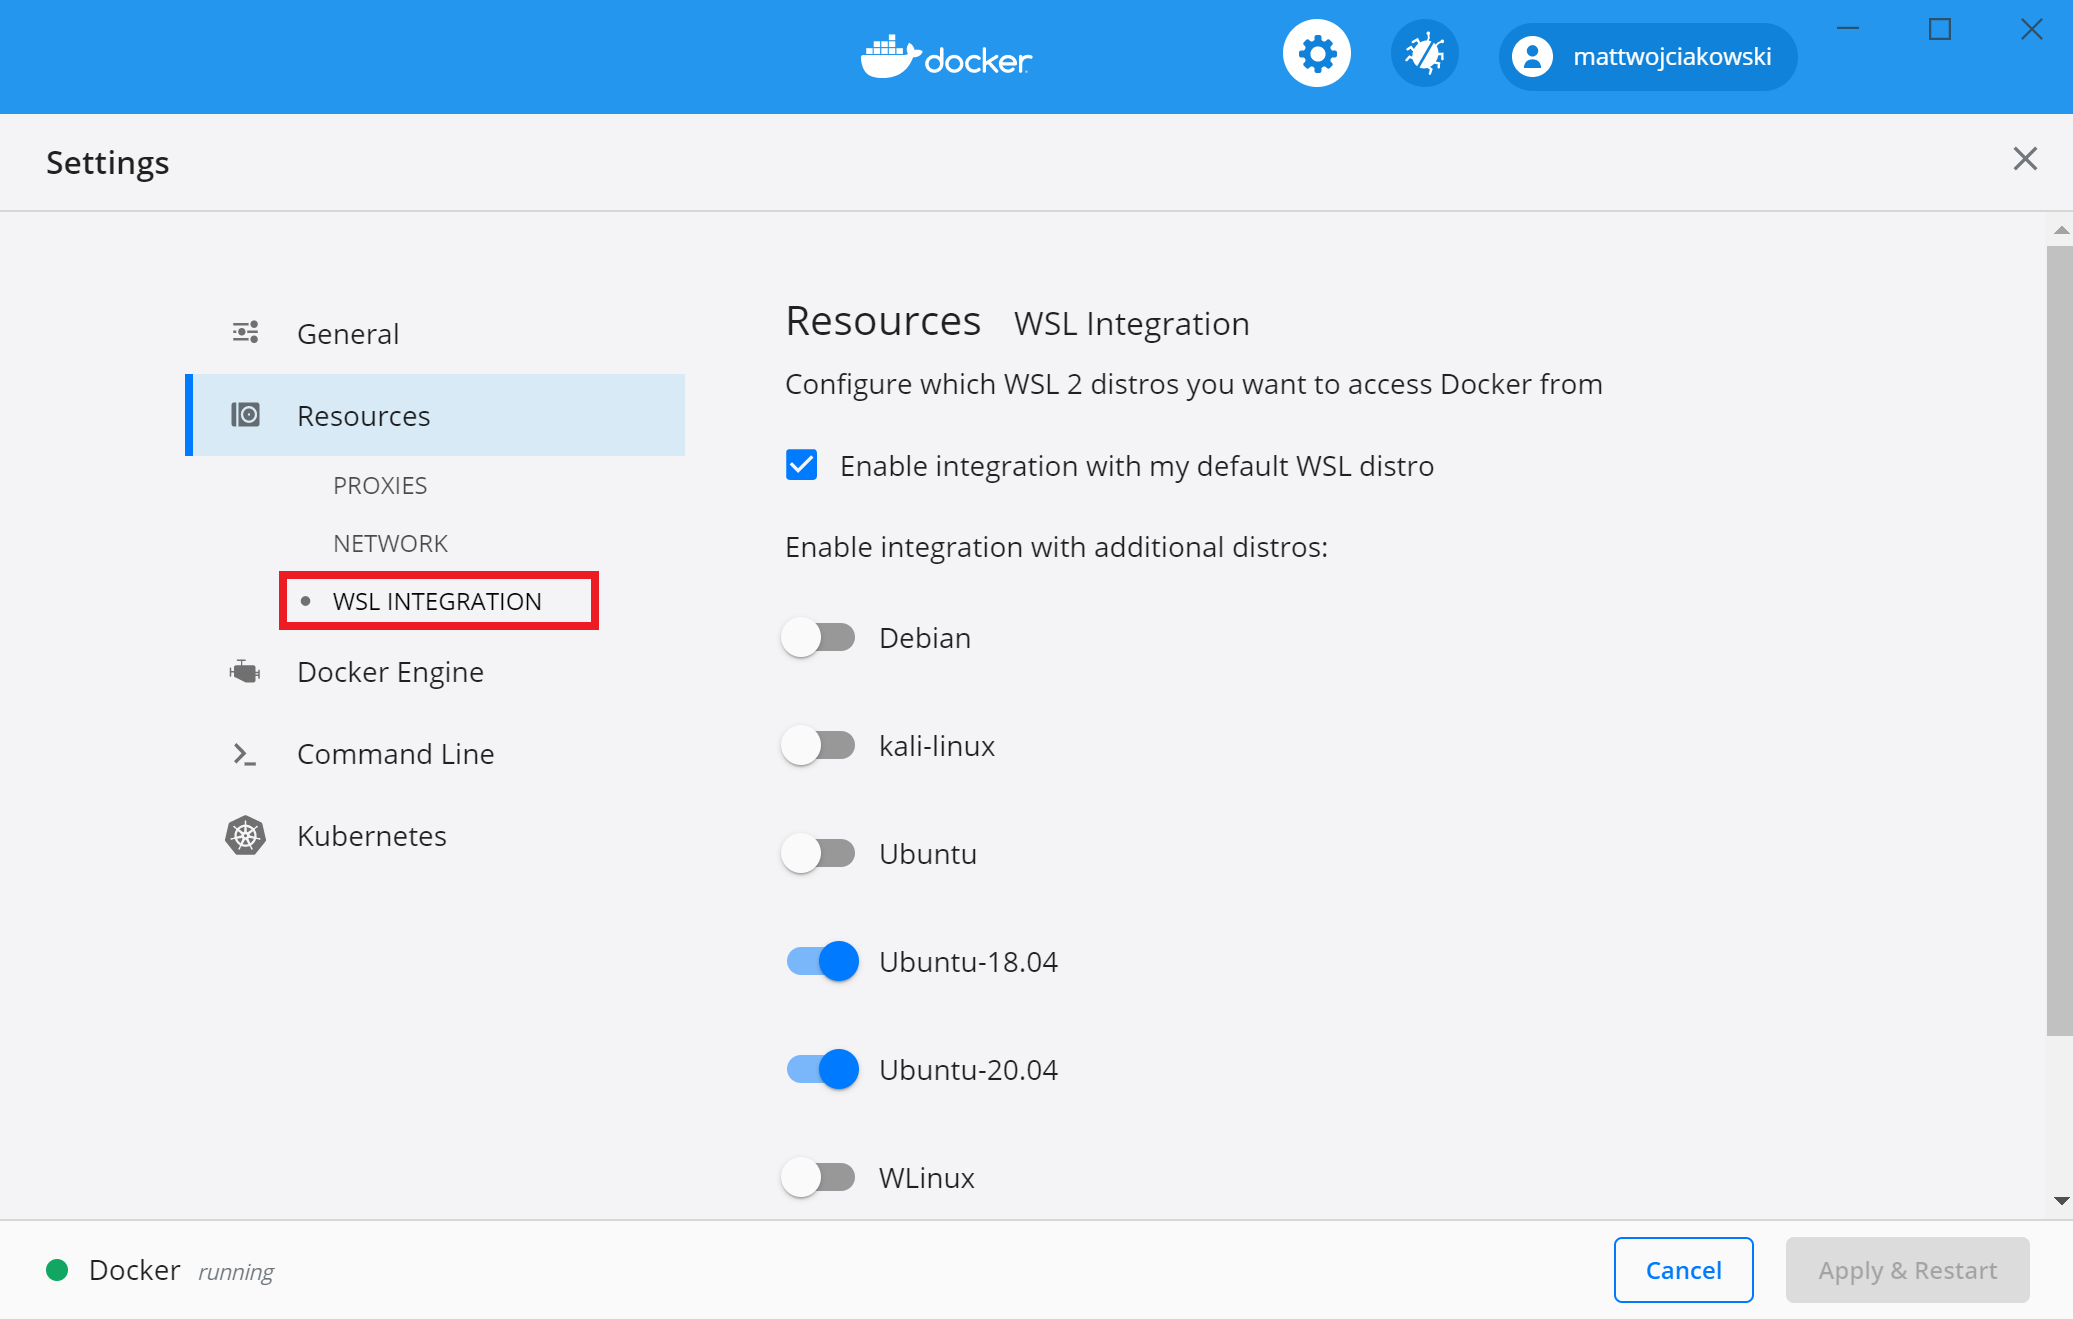
\includegraphics[width=\textwidth]{img/docker-dashboard.png}  
    \caption{Ventana de docker para habilitar WSL. Imagen extraída de \url{https://learn.microsoft.com/es-es/windows/wsl/tutorials/wsl-containers}}  
    \label{fig:dockerdashboard}
\end{figure}


\subsection{Preparación de DevContainer}

Desde Visual Studio Code se puede abrir el contenido del proyecto correspondiente a la carpeta \texttt{/Mazmorras}. Para hacerlo en la esquina superior derecha como se muestra en la figura \ref{fig:FileVS}.

Una vez abierto se necesita descargar la extensión \texttt{Dev Containers}. Para hacerlo en la barra de menú que se encuentra en el margen derecho se debe ir al botón que se muestra en la figura \ref{fig:Extensiones}.
La extensión es la que se muestra en la figura \ref{fig:DevContainers}.

\begin{figure}[!h]  
    \centering  
    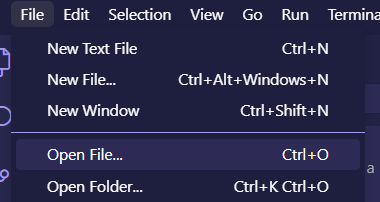
\includegraphics[width=\textwidth]{img/FileVS.png}  
    \caption{Pestaña de archivos en Visual Studio Code}  
    \label{fig:FileVS}
\end{figure}
\begin{figure}[!h]  
    \centering  
    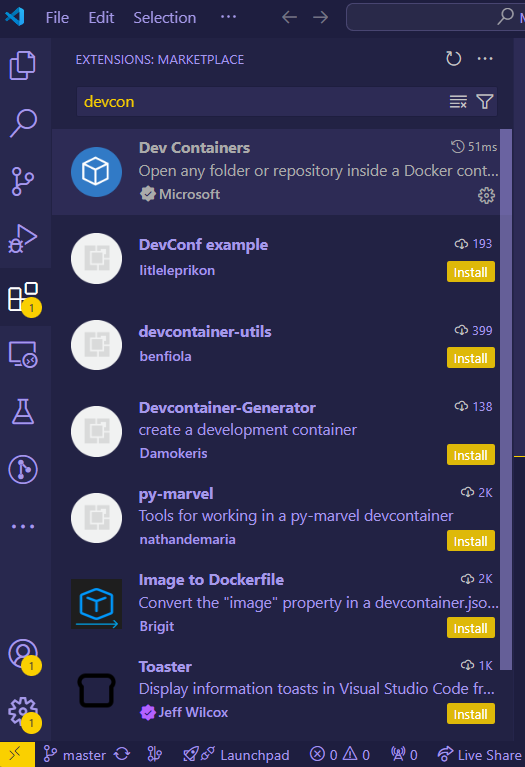
\includegraphics[width=\textwidth]{img/Extensiones.png}  
    \caption{Pestaña extensiones en Visual Studio Code}  
    \label{fig:Extensiones}
\end{figure}
\begin{figure}[!h]  
    \centering  
    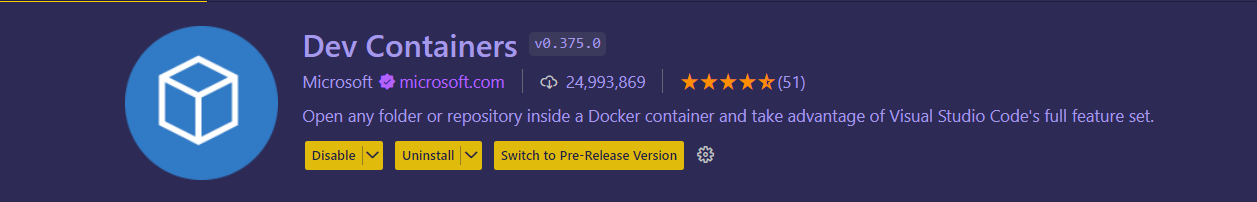
\includegraphics[width=\textwidth]{img/devcontainersextension.png}  
    \caption{Pestaña de la extensión Dev Containers en Visual Studio Code}  
    \label{fig:DevContainers}
\end{figure}

Al instalar la extensión, automáticamente aparece la notificación de la figura \ref{fig:opencontainer}, al pulsar en el botón de <<Reopen in container>> volverá a abrir el proyecto, esta vez desde el contenedor ya preparado.

\begin{figure}[!h]  
    \centering  
    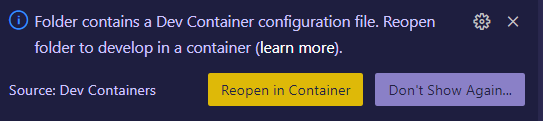
\includegraphics[width=\textwidth]{img/reopencontainer.png}  
    \caption{Notificación de reapertura de proyecto como Dev Container}  
    \label{fig:opencontainer}
\end{figure}

Si no apareciese la notificación, se puede abrir con la extensión siguiendo los siguientes pasos. Primero se necesita pulsar el botón para abrir el proyecto desde una ventana remota, como se muestra en la figura \ref{fig:botoncontainer}. Tras esto se abrirá el menú de selección como se muestra en la figura \ref{fig:remoteWindow}. Se necesita seleccionar la opción <<Reopen in Container>>, al hacerlo se volverá a abrir el proyecto desde el contenedor.

\begin{figure}[!h]  
    \centering  
    
\includegraphics{img/botoncontainer.png}  
    \caption{Botón para ejecutar la apertura de una ventana remota}  
    \label{fig:botoncontainer}
\end{figure}

\begin{figure}[!h]  
    \centering  
    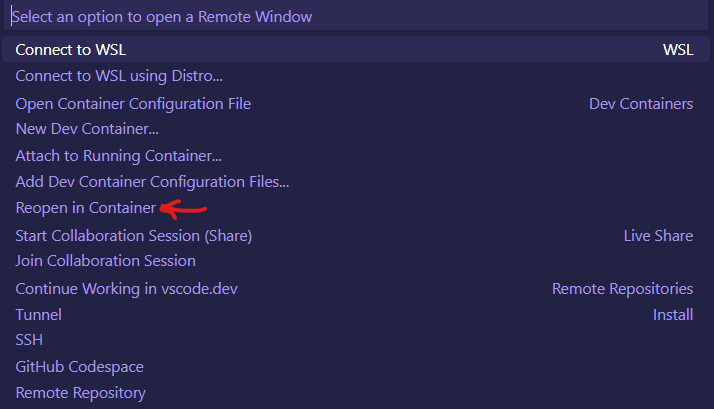
\includegraphics[width=\textwidth]{img/reopencontainerdevcontainer.png}  
    \caption{Menú de ejecución de ventana remota}  
    \label{fig:remoteWindow}
\end{figure}

\subsection{Levantar el servidor}

Para levantar el servidor se aconseja usar la terminal integrada de Visual Studio Code, esta se puede abrir desde la barra superior de la ventana como se muestra en la figura \ref{fig:terminal}.
\begin{figure}[!h]  
    \centering  
    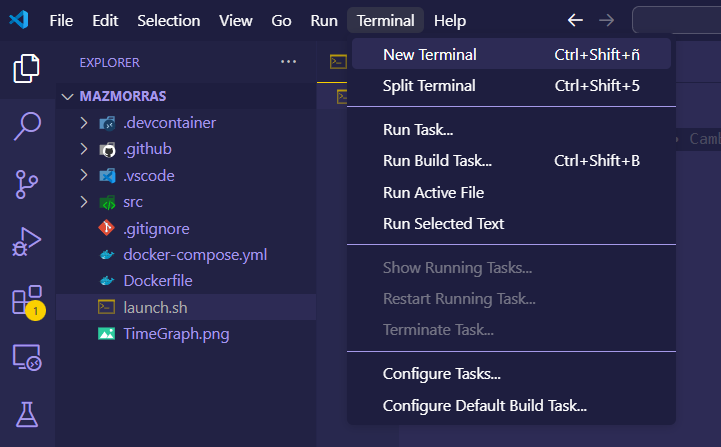
\includegraphics[width=\textwidth]{img/terminal.png}  
    \caption{Barra de opciones de Visual Studio Code}  
    \label{fig:terminal}
\end{figure}

El servidor de laberintos se lanza a través de un contendor de Docker, siguiendo la configuración especificada en el Dockerfile. Para poder hacerlo tenemos que introducir en la terminal en la ruta del directorio del backend el siguiente comando: 
\begin{lstlisting}
    docker compose up
\end{lstlisting}
Se lanzarán un contenedor con el servidor y otro de mongo, siguiendo la configuración del fichero Docker-compose.yml contenida en ese directorio.

Para poder parar el contenedor, desde el teclado se pulsarían los botones Ctrl+C y para borrar el contenedor se realiza con el siguiente comando:
\begin{lstlisting}
    docker compose down
\end{lstlisting}



\section{Pruebas del sistema}
Es necesario para asegurar una buena experiencia de usuario poner el sistema desarrollado a prueba. En el caso de este proyecto, está compuesto de dos partes que necesitan pruebas distintas.

Para realizar pruebas que comprueben el funcionamiento del servidor, se realizaron pruebas de peticiones predefinidas y respuestas esperadas, en este caso la herramienta elegida fue Postman\footnote{Esta herramienta permite comprobar el correcto funcionamiento de una API a través de llamadas predefinidas, para más información \url{https://learning.postman.com/docs/introduction/overview/}}.

Para comprobar el correcto funcionamiento del videojuego, se han preparado ejecutables que después se han testeado, a este proceso se le llama beta testeo. Se recomienda que este testeo lo realicen personas no familiarizadas con el proyecto, estas probarán el videojuego para poder encontrar problemas que el desarrollador no podría encontrar. El proceso de beta testeo fue esencial para obtener una experiencia de usuario adecuada.


\apendice{Documentación de usuario}

\section{Introducción}
En esta sección se va a desarrollar el uso que se puede hacer de la aplicación por parte del usuario.
Este proyecto se compone de dos partes, un ejecutable y el servidor. 

\section{Requisitos de usuarios}

Este proyecto en el estado en el que se encuentra ahora se necesita arrancar el servidor en la máquina localmente pero en líneas futuras, esto no sería necesario para el usuario ya que está preparado para ser alojado en un servidor externo.

A continuación se van a presentar los requisitos que se necesita por parte del usuario: 
\begin{itemize}
    \item \textbf{Sistema operativo}: Debe de tener un sistema operativo Windows 10 o superior o Linux Ubuntu 18.04 o superior
    \item \textbf{Procesador}: Intel Core i3 o equivalente
    \item \textbf{Memoria RAM}: 4GB
    \item \textbf{Espacio en el disco}: Al menos 64GB de espacio libre
\end{itemize}

\section{Instalación}

Para poder ejecutar el proyecto en el dispositivo, se necesita instalar el Docker para poder arrancar el servidor en local. El proceso de instalación es igual a lo mencionado anteriormente en el manual del programador.
Se necesita descargar el repositorio de la siguiente url \url{https://github.com/etc99/algoritmosYmazmorras}.

\section{Manual del usuario}

\subsection{Manual del servidor}

Para poder visualizar los laberintos en el juego, primero es necesario tener arrancado el servidor. 
Para realizarlo es necesario abrir la terminal. 

En la terminal, con la ruta del directorio apuntando a \texttt{/Mamzmorras} se necesita ejecutar el siguiente comando para levantar el servidor:
\begin{lstlisting}
    docker compose up
\end{lstlisting}

Para poder parar el contenedor del juego, desde el teclado se pulsarían los botones Ctrl+C y para borrar el contenedor se realiza con el siguiente comando:
\begin{lstlisting}
    docker compose down
\end{lstlisting}

\subsection{Manual del juego}
Teniendo ya listo el servidor, ahora solo queda lanzar el ejecutable del videojuego. En la carpeta del ejecutable aparecerán diversos archivos, pero el ejecutable es el que se encuentra marcado en la figura \ref{fig:EjecutableUnity}.

\begin{figure}[!h]  
    \centering  
    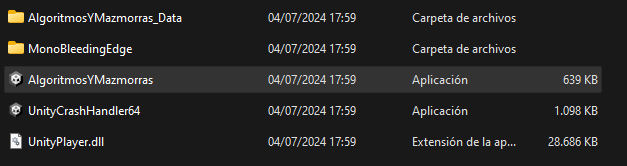
\includegraphics[width=\textwidth]{img/EjecutableUnity.png}  
    \caption{Carpeta del ejecutable de Unity.}  
    \label{fig:EjecutableUnity}
\end{figure}

Tras esto la primera pantalla que se mostrará es el menú principal como se muestra en la figura \ref{fig:MenuPrincipal}. Para poder avanzar a la siguiente pantalla se necesita pulsar sobre el botón de <<¡Comenzar!>>, al hacerlo se muestra la pantalla de selección de algoritmo \ref{fig:MenuSeleccion}.

Tras seleccionar uno de los algoritmos en la siguiente se mostrará lo que va a ser el tablero y el jugador, y en el margen izquierdo aparecerá un menú en el que se podrán introducir los parámetros deseados para el laberinto \ref{fig:ParametrosLaberinto}.

Después de introducir los parámetros se pulsa sobre el botón de <<Generar>>. Tras realizar esto se muestra el resultado para poder navegar el laberinto con las teclas <<W, A, S, D>> \ref{fig:LaberintoGenerado}.


\begin{figure}[!h]  
    \centering  
    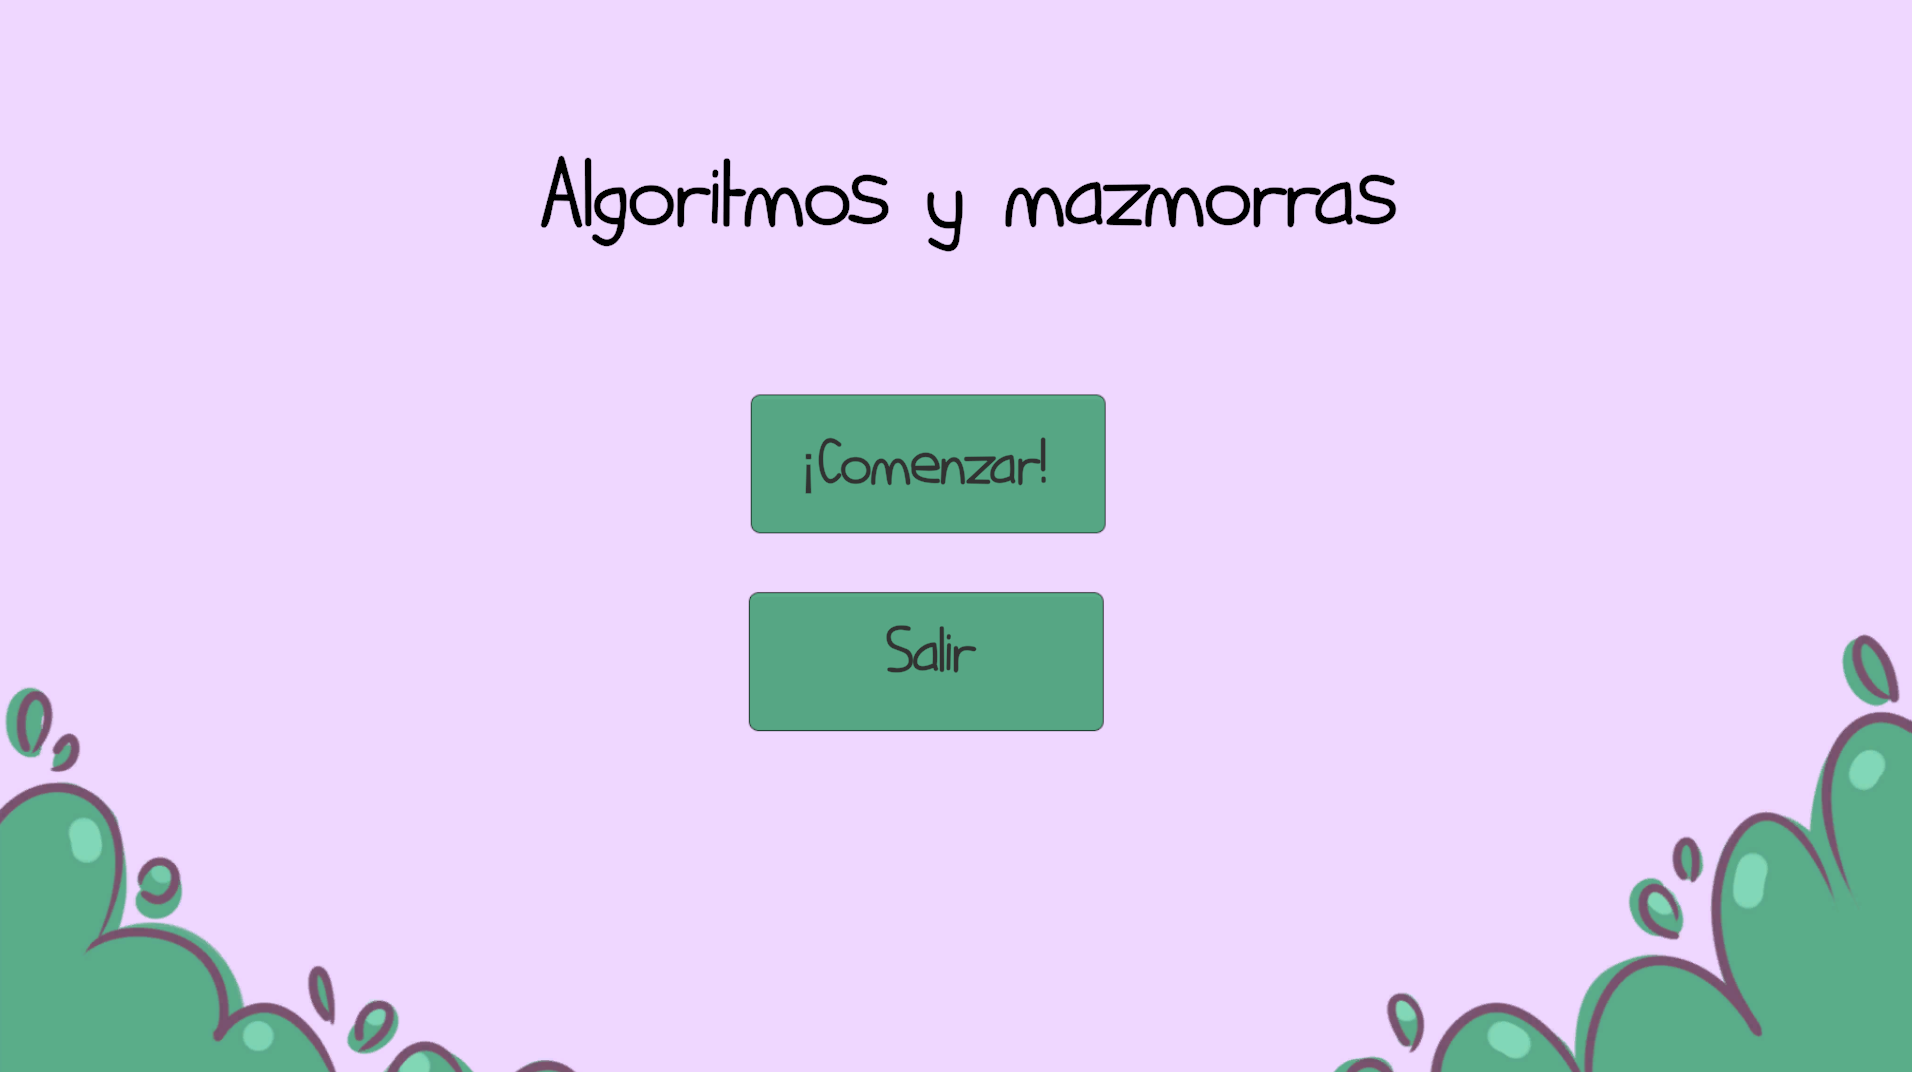
\includegraphics[width=\textwidth]{img/MenuPrincipal.png}  
    \caption{Captura del menú principal del juego.}  
    \label{fig:MenuPrincipal}
\end{figure}

\begin{figure}[!h]  
    \centering  
    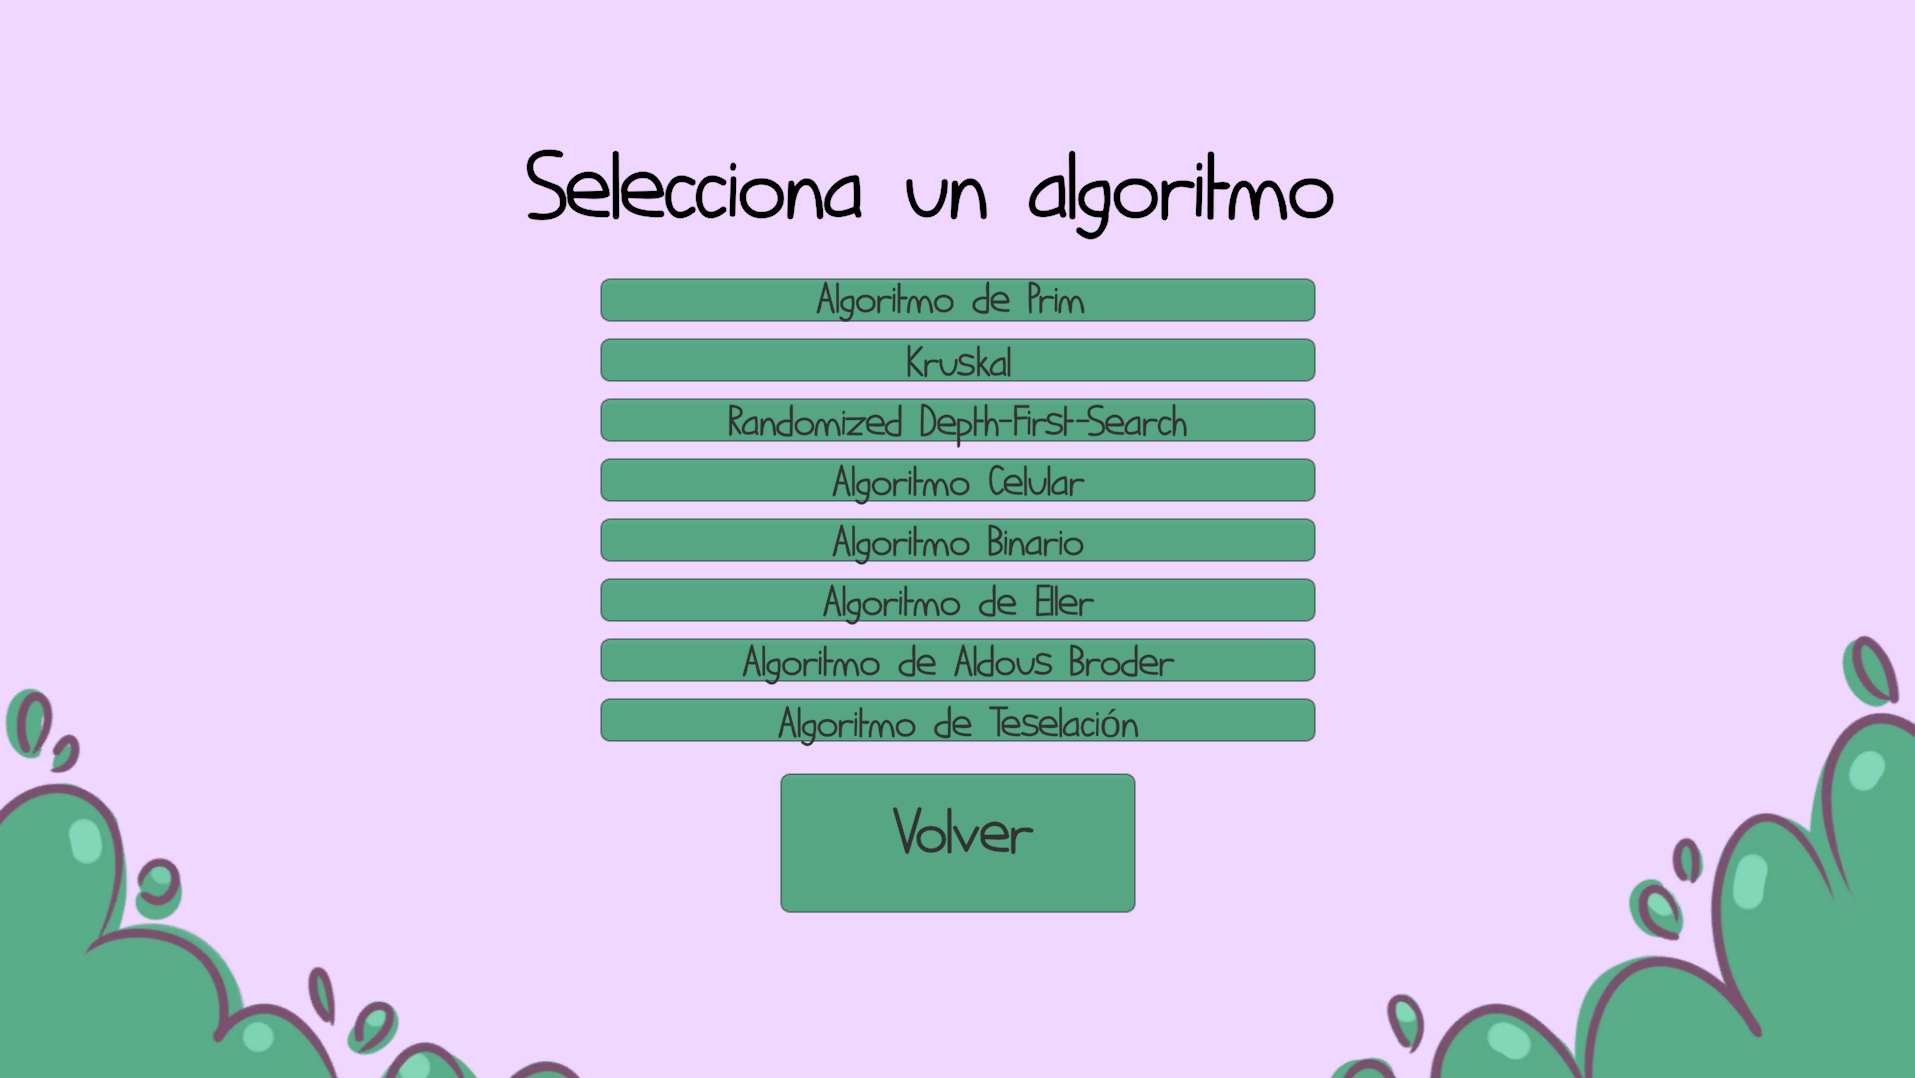
\includegraphics[width=\textwidth]{img/MenuSeleccion.png}  
    \caption{Captura del menú de selección de algoritmo.}  
    \label{fig:MenuSeleccion}
\end{figure}

\begin{figure}[!h]  
    \centering  
    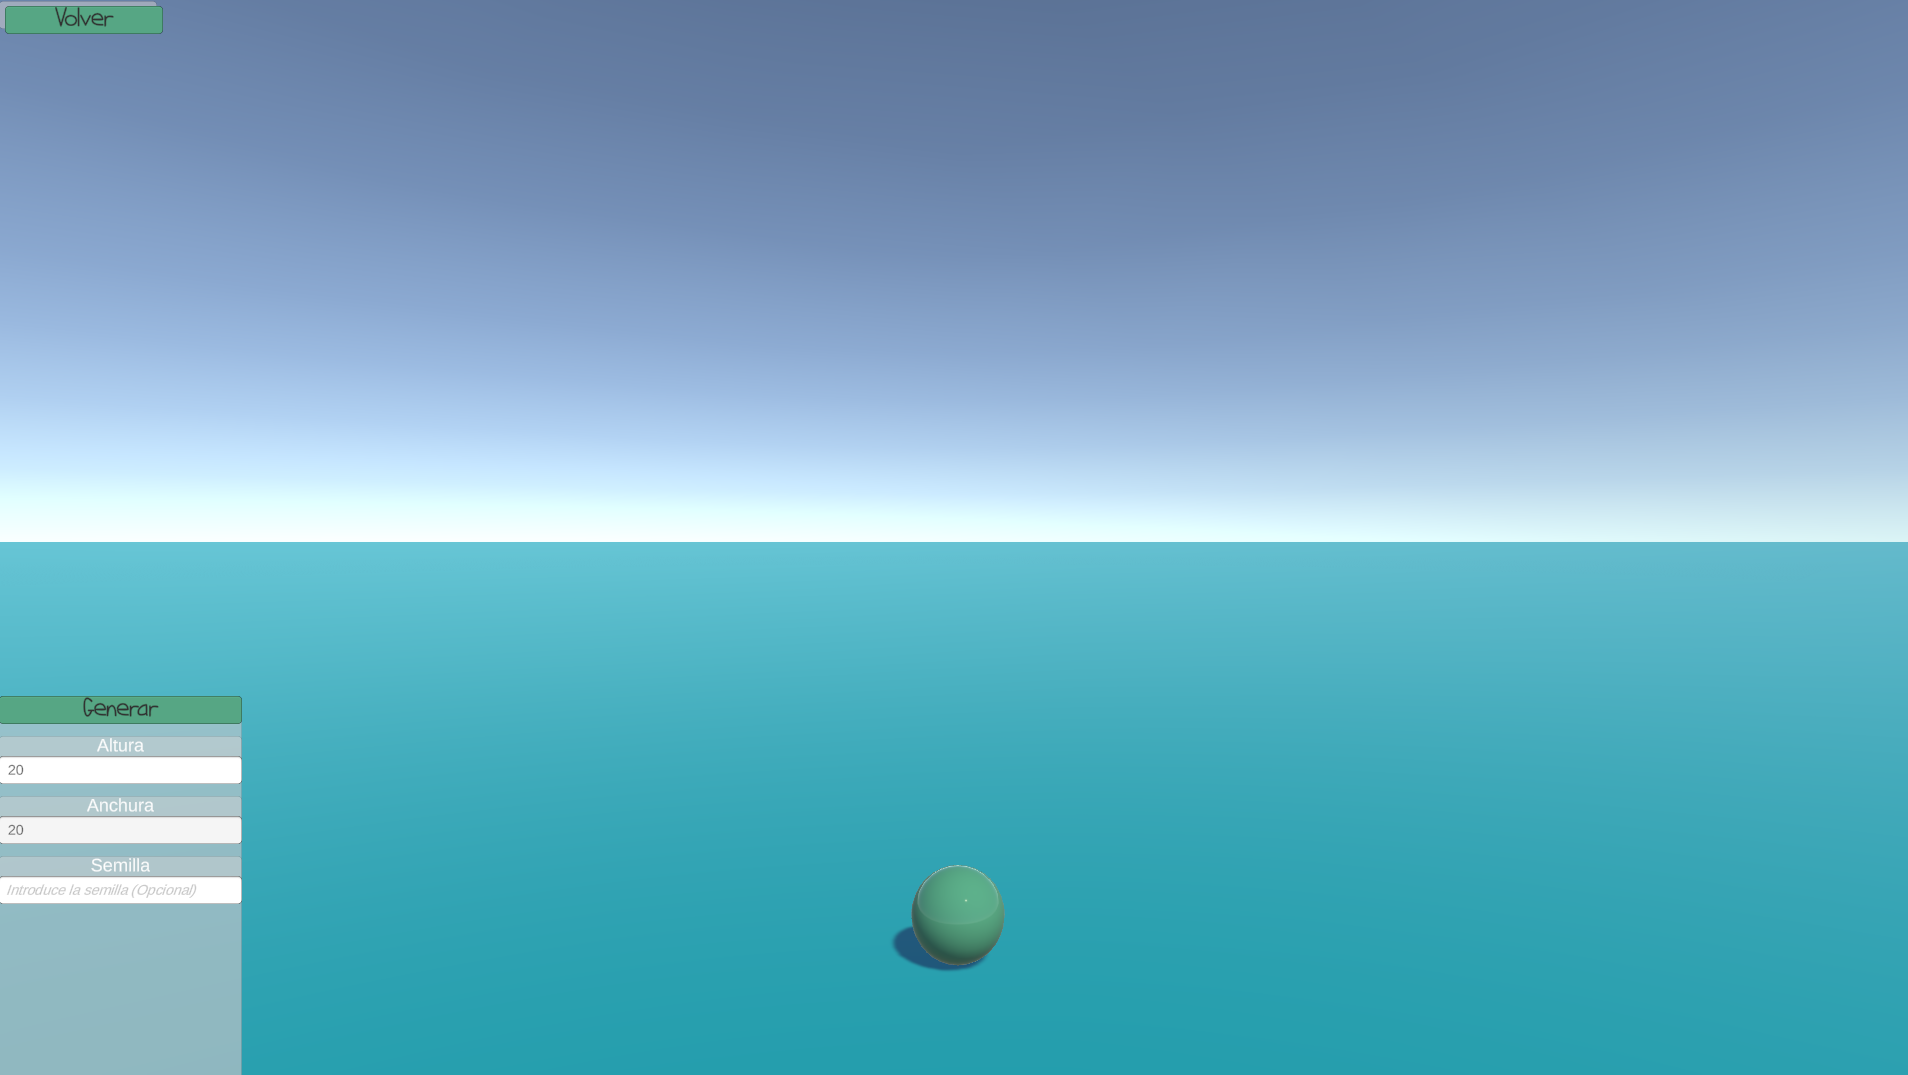
\includegraphics[width=\textwidth]{img/IntroducirParametrosLaberinto.png}  
    \caption{Captura de la interfaz para introducir los parámetros del laberinto.}  
    \label{fig:ParametrosLaberinto}
\end{figure}

\begin{figure}[!h]  
    \centering  
    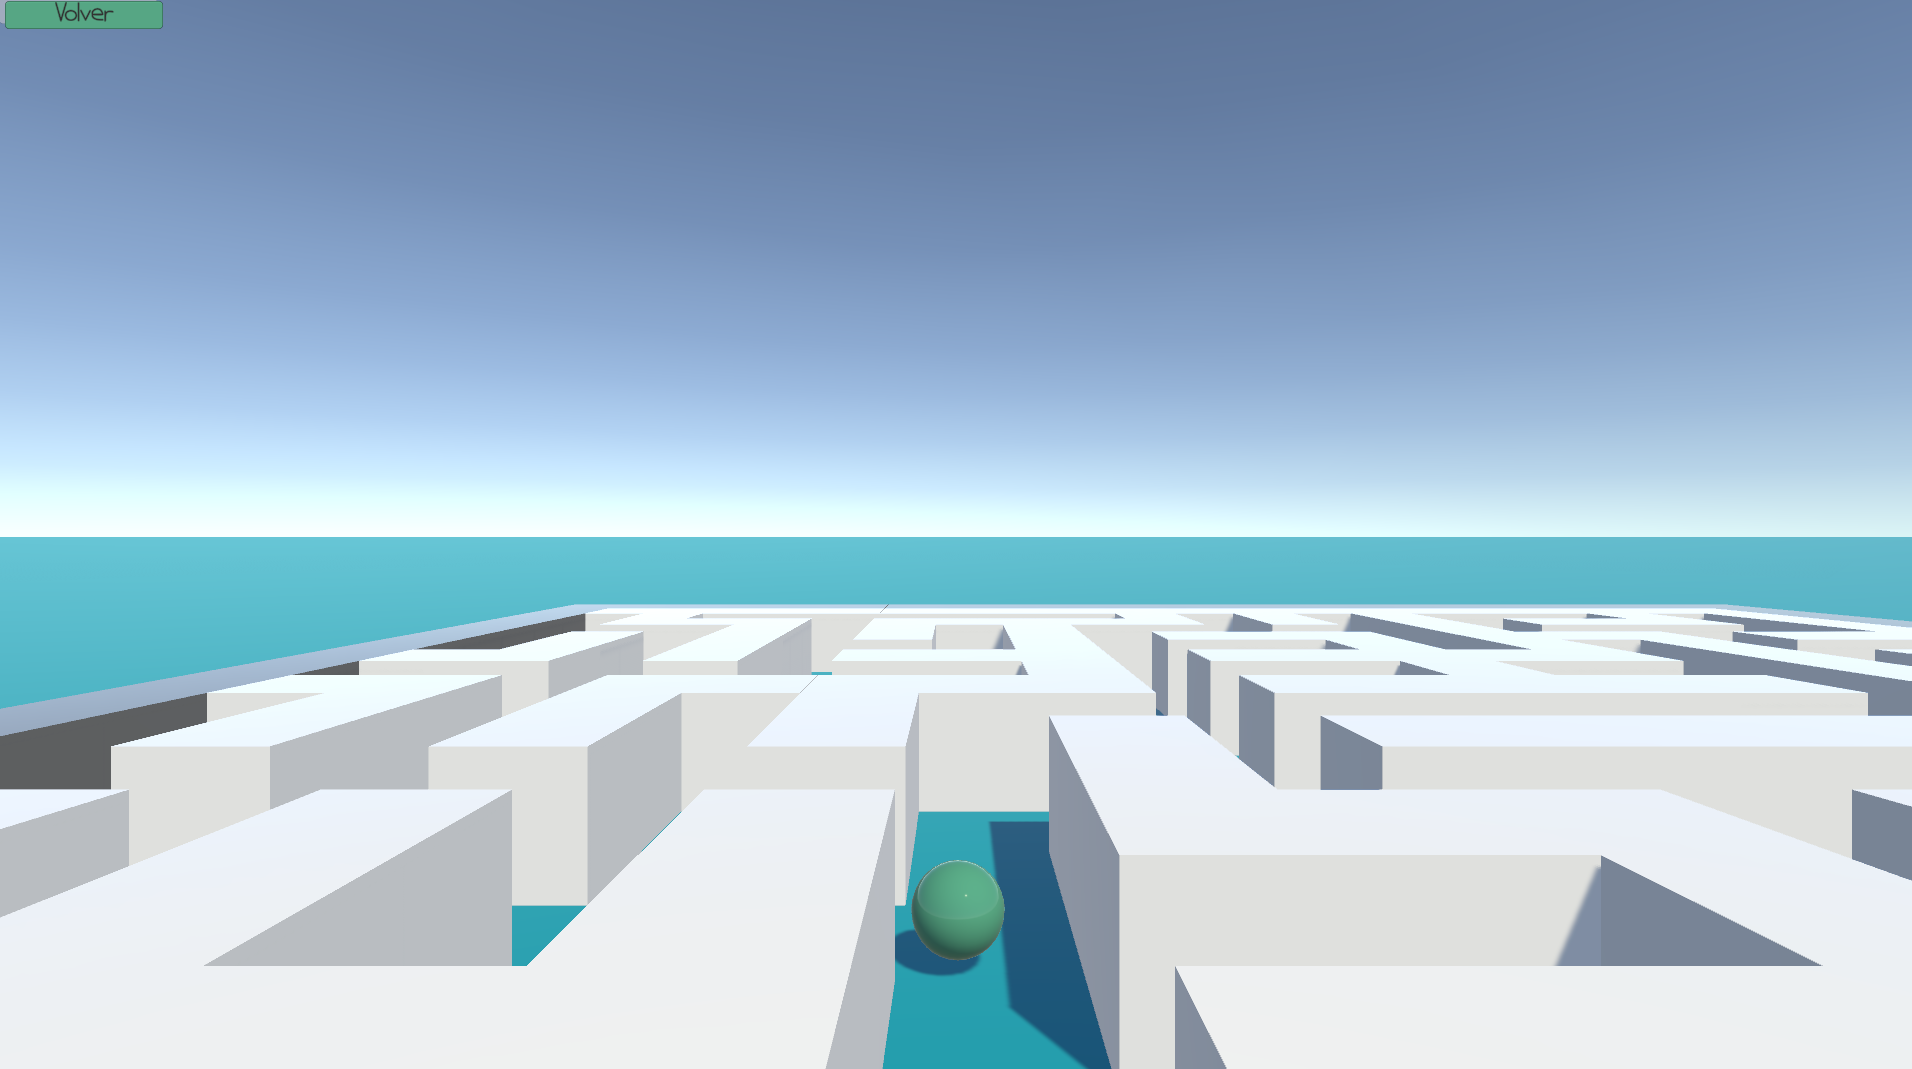
\includegraphics[width=\textwidth]{img/LaberintoGenerado.png}  
    \caption{Captura del laberinto generado.}  
    \label{fig:LaberintoGenerado}
\end{figure}
\apendice{Sostenibilización curricular}

\section{Introducción}
El documento ``Directrices para la introducción de la Sostenibilidad en el Curriculum'' aprobado por la CRUE establece una serie de objetivos clave para la integración de la sostenibilidad en el currículo de las universidades españolas. Estos objetivos tienen como propósito fundamental fomentar un desarrollo humano sostenible a través de la educación superior. A continuación, se detallan los principales objetivos planteados:

\section{Integración Transversal de la Sostenibilidad}
\textbf{Objetivo:} Incluir la sostenibilidad como un eje transversal en todas las titulaciones universitarias, asegurando que todos los estudiantes adquieran competencias en este ámbito, independientemente de su área de estudio.\\
\textbf{Acciones:} Se promoverá la revisión y actualización de los planes de estudio para incluir contenidos específicos y transversales sobre sostenibilidad, adaptados a cada disciplina.

\section{Desarrollo de Competencias para la Sostenibilidad}
\textbf{Objetivo:} Desarrollar en los estudiantes las competencias necesarias para identificar y resolver problemas socioambientales desde una perspectiva sistémica y ética.\\
\textbf{Acciones:} Los planes de estudio deberán contemplar la formación en competencias como el pensamiento crítico, la gestión sostenible de recursos, la participación en procesos comunitarios y la aplicación de principios éticos en la vida personal y profesional.

\section{Fomento de la Investigación y Docencia Sostenible}
\textbf{Objetivo:} Promover la investigación y la docencia que integren los principios del desarrollo sostenible, asegurando que la actividad académica contribuya a la solución de problemas ambientales y sociales.\\
\textbf{Acciones:} Se incentivará la realización de proyectos de investigación y la impartición de cursos que aborden la sostenibilidad desde diversas perspectivas, facilitando la formación continua y el aprendizaje a lo largo de la vida.

\section{Sensibilización y Participación de la Comunidad Universitaria}
\textbf{Objetivo:} Involucrar a toda la comunidad universitaria en el compromiso con la sostenibilidad, fomentando la participación activa en la implementación de políticas y acciones sostenibles dentro y fuera del campus.\\
\textbf{Acciones:} Se promoverán actividades extracurriculares, seminarios, talleres y jornadas que sensibilicen a estudiantes, profesores y personal administrativo sobre la importancia de la sostenibilidad y su aplicación en la vida diaria.

\section{Establecimiento de Mecanismos de Evaluación y Mejora Continua}
\textbf{Objetivo:} Implementar sistemas de evaluación que aseguren la calidad y efectividad de las acciones educativas en sostenibilidad, permitiendo una mejora continua de los programas académicos y las prácticas institucionales.\\
\textbf{Acciones:} Se incluirán criterios de sostenibilidad en los sistemas de evaluación de la calidad universitaria y en la evaluación del profesorado, garantizando que tanto la docencia como la investigación se alineen con los principios del desarrollo sostenible.

\section{Creación de Redes y Plataformas de Colaboración}
\textbf{Objetivo:} Establecer redes de colaboración entre universidades y otras entidades para intercambiar experiencias y buenas prácticas en la integración de la sostenibilidad en el currículo académico.\\
\textbf{Acciones:} Se fomentará la creación de grupos de trabajo interuniversitarios y la participación en plataformas estatales e internacionales que faciliten el intercambio de conocimientos y la cooperación en proyectos de sostenibilidad.

Estos objetivos buscan no solo la formación de profesionales capacitados para enfrentar los desafíos actuales y futuros, sino también la creación de una cultura universitaria comprometida con la sostenibilidad y el desarrollo humano integral. La implementación efectiva de estas directrices requiere del compromiso institucional y la participación activa de toda la comunidad universitaria.\cite{crue2020}




\bibliographystyle{plain}
\bibliography{bibliografiaAnexos}

\end{document}
